\anexo{INFORMAÇÕES CADASTRAIS}

\newpage
\begin{center}
\textbf{INFORMAÇÕES CADASTRAIS}
\addcontentsline{toc}{chapter}{INFORMAÇÕES CADASTRAIS}
\end{center}
\begin{SingleSpace}

\textbf{Razão Social:} QSE Consultoria e Assessoria LTDA. 

\textbf{Endereço:} Rua Pio Antônio de Oliveira, 92 \\

\textbf{Bairro:} Pacaembu \textbf{Cidade:} Uberlândia \textbf{Estado:} MG \textbf{CEP:} 38401-482 \\

\textbf{CNPJ:} 17.533.344/0001-69 \\

\textbf{Insc. Est.:} ISENTO \\

Ramo de atividade: Prestação de serviços de consultoria e assessoria em Engenharia Química, de Segurança do Trabalho e do Meio Ambiente, envolvendo projetos, perícias, laudos técnico, medições e treinamentos. \\

\textbf{RESPONSÁVEL TECNICO}
Eng. Químico Dr. Euclides Antônio Pereira de Lima CRQ-MG: 02301286 II-Região/CREA – MG: 088801-D \\

Participação em cursos afins:

\begin{enumerate}
\begin{scriptsize}
	\item AMOSTRAGEM EM DUTOS E CHAMINÉS – 19 a 25/05/2003 – CETESBSP Certificado no 007/2003 \\
	\item TÉCNICAS DE AMOSTRAGEM E ANÁLISE DE POLUENTES NA ATMOSFERA 07 a 10/10/2002 -  CETESB  SP Certificado no 044/2002 \\
	\item TECNOLOGIAS E SELEÇÃO DE SISTEMAS DE CONTROLE DA POLUIÇÃO DO AR: MATERIAL PARTICULADO, GASES, VAPORES E ODORES – 26 a 28/08/2002 -CETESB  SP Certificado no 0695/2002 \\
	\item IMPLANTAÇÃO DA NBR ISO/IEC 17025:2005 – com carga horária de 24 horas – JOROM Prestação de Serviço em Consultoria Tecnológica LTDA. – Curso Autorizado pela Secretária de Estado da Educação e do Desporto – SC – PORTARIA Nº 008 de 25/06/2002. \\
	\item AUDITOR INTERNO DA ABNT NBR ISO/IEC 17025:2005 – 20 a 22/03/2009 com carga horária de 20 horas – JOROM Prestação de Serviço em Consultoria Tecnológica LTDA. – Curso Autorizado pela Secretária de Estado da Educação e do Desporto – SC – PORTARIA Nº 008 de 25/06/2002.
	\item AUDITOR INTERNO SAÚDE E SEGURANÇA OCUPACIONAL OHSAS 18001:2007 – 20 a 22/11/2009 – com carga horária de 24 horas – INBRAFORP – Certificado nº 000105/2009. \\
	\item ESTIMATIVA DE EMISSÕES DE POLUENTES ATMOSFÉRICOS – de 04 a 07/05/2010 – com carga horária de 28 horas – CETESB  SP. \\
	\item Utilização do medidor de nível de pressão sonora Solo SLM com carga horária de 4 horas ministrado  pela 01 dB Brasil \\
	\item Aplicação da norma NBR 10151 / 2000 ao controle do ruído no meio ambiente: Conceitos, procedimentos e uso de instrumentos de medição com carga de 16 horas, ministrado por João Gualberto de Azevedo Baring. \\
\end{scriptsize}
\end{enumerate}

\end{SingleSpace}


\anexo{LAUDO DE CALIBRAÇÃO DO CALIBRADOR ACÚSTICO}

\newpage

\

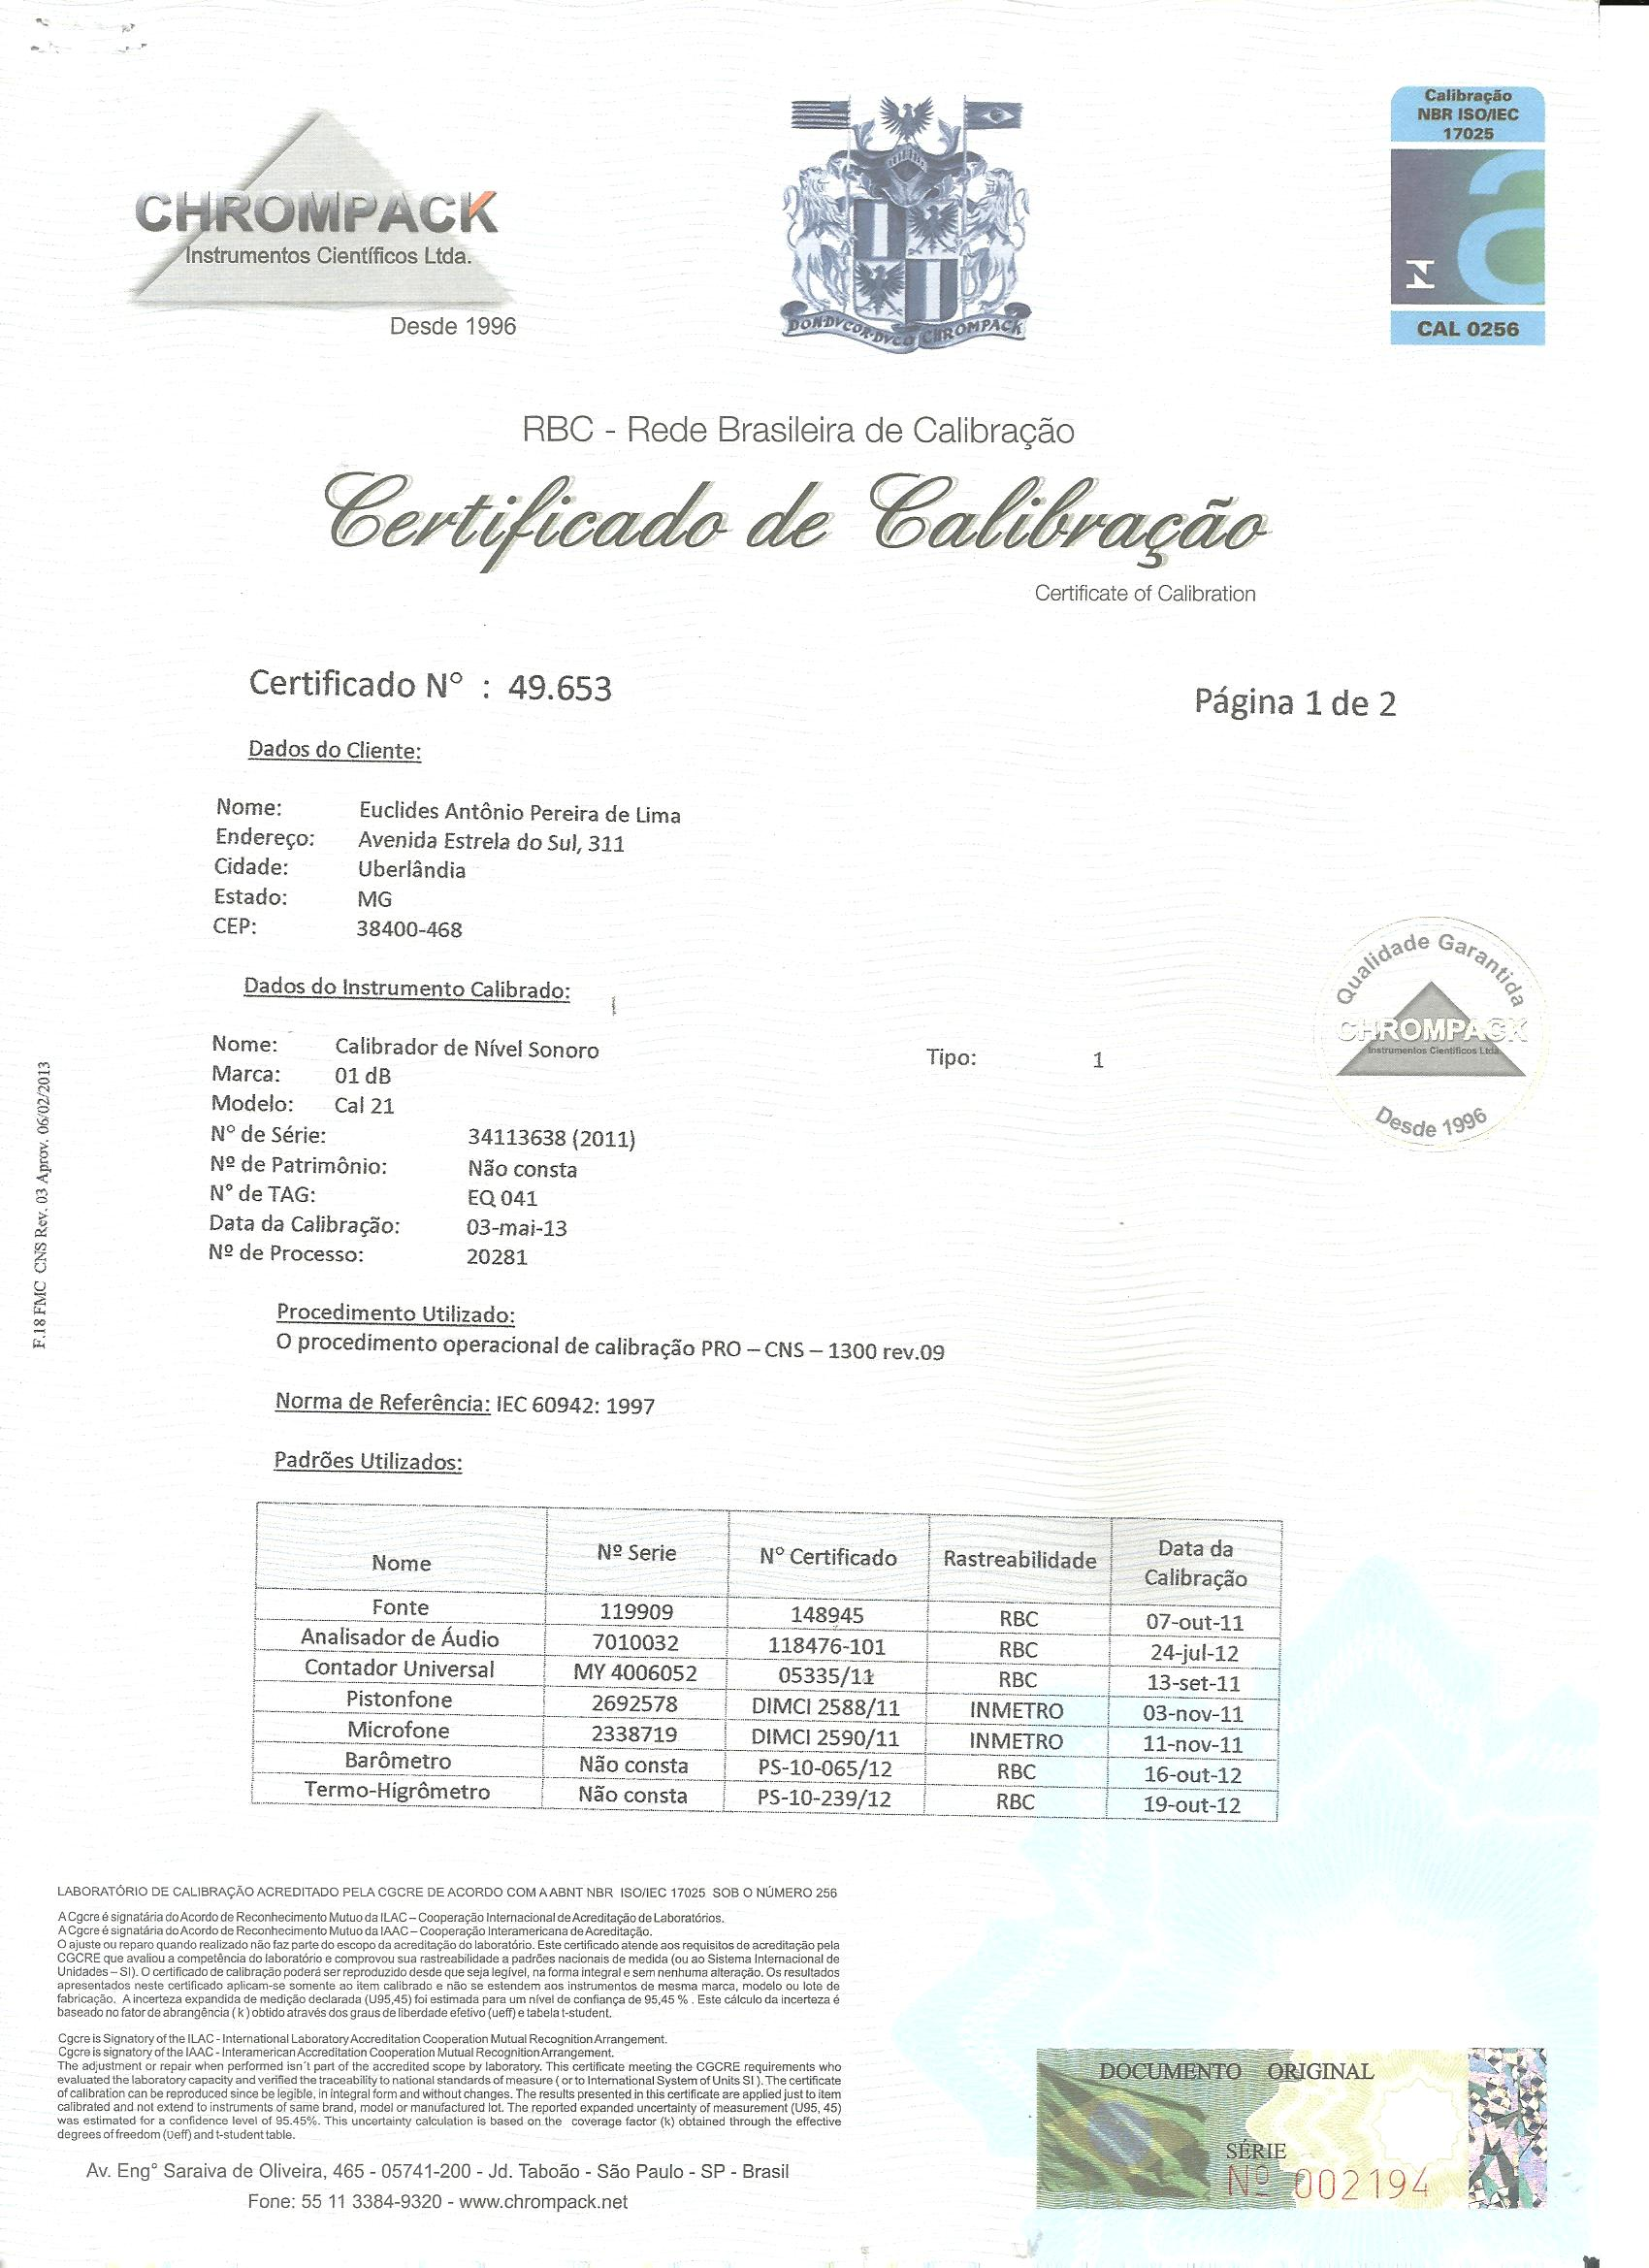
\includegraphics[width=0.9\linewidth]{temp/imagens/anexo2/01.jpg}
\newpage

\

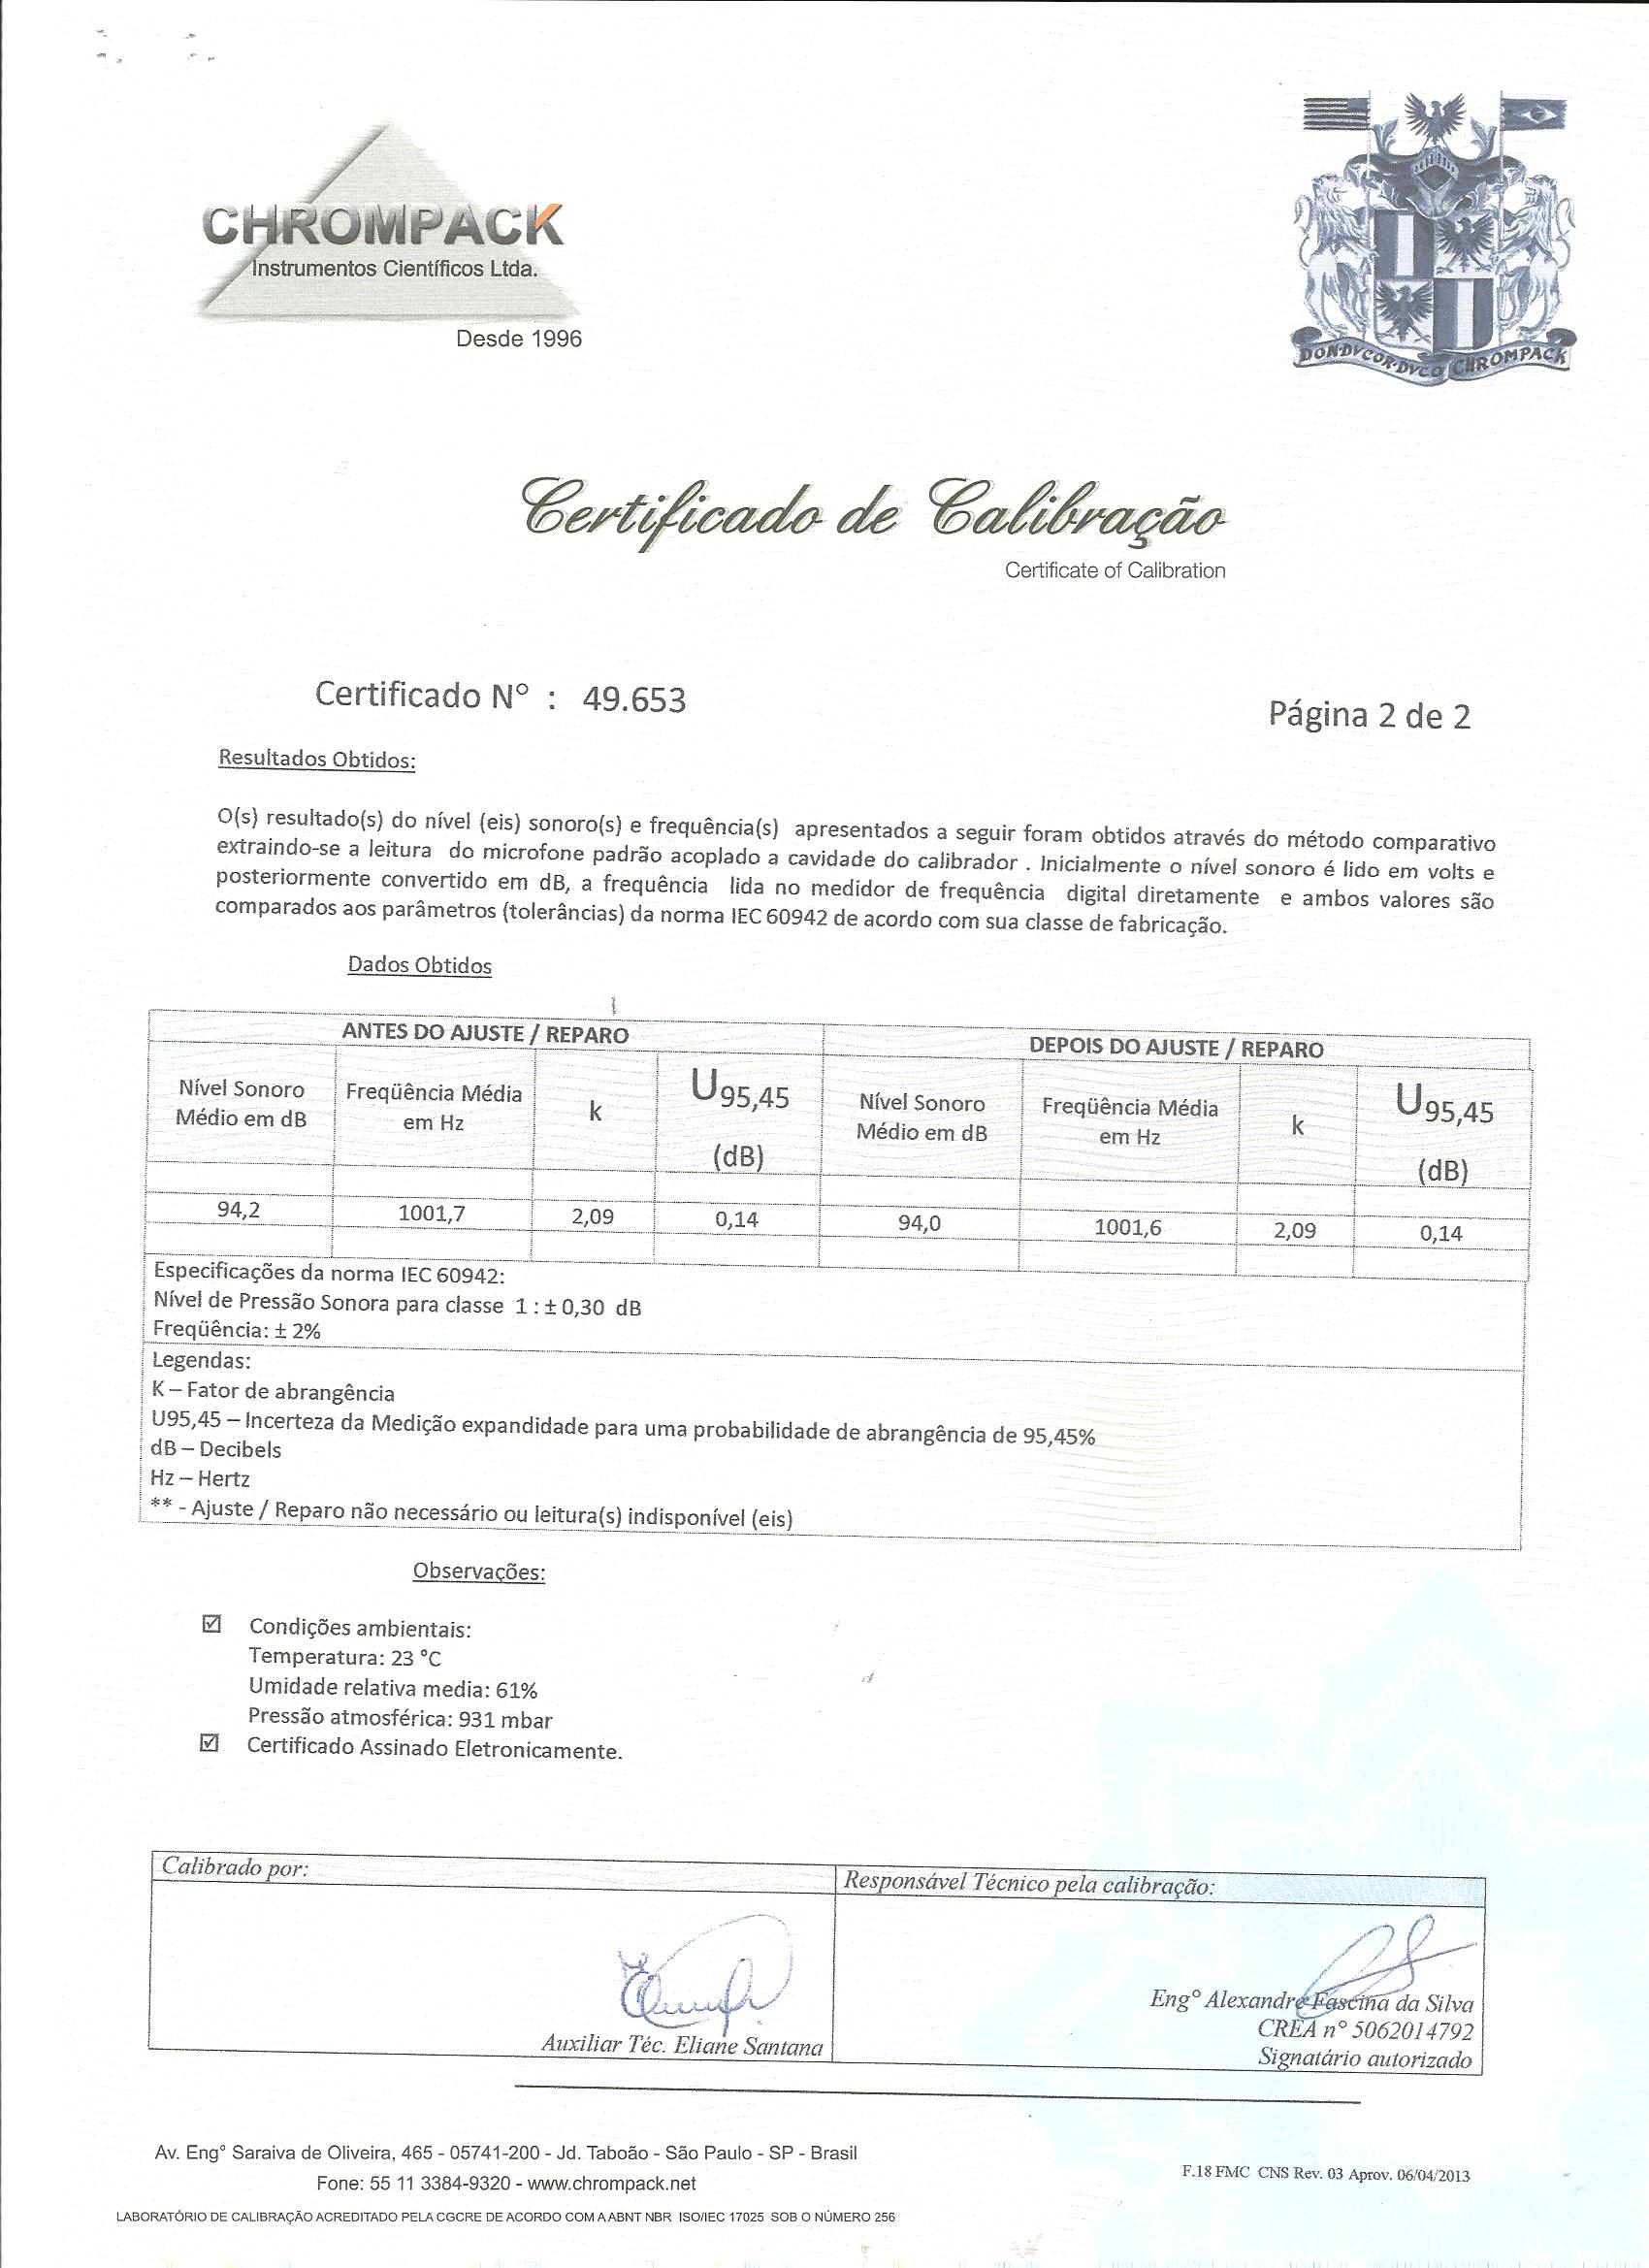
\includegraphics[width=0.9\linewidth]{temp/imagens/anexo2/02.jpg}
\anexo{LAUDO DE CALIBRAÇÃO DO MEDIDOR INTEGRADOR DE RUÍDO}

\

\

\

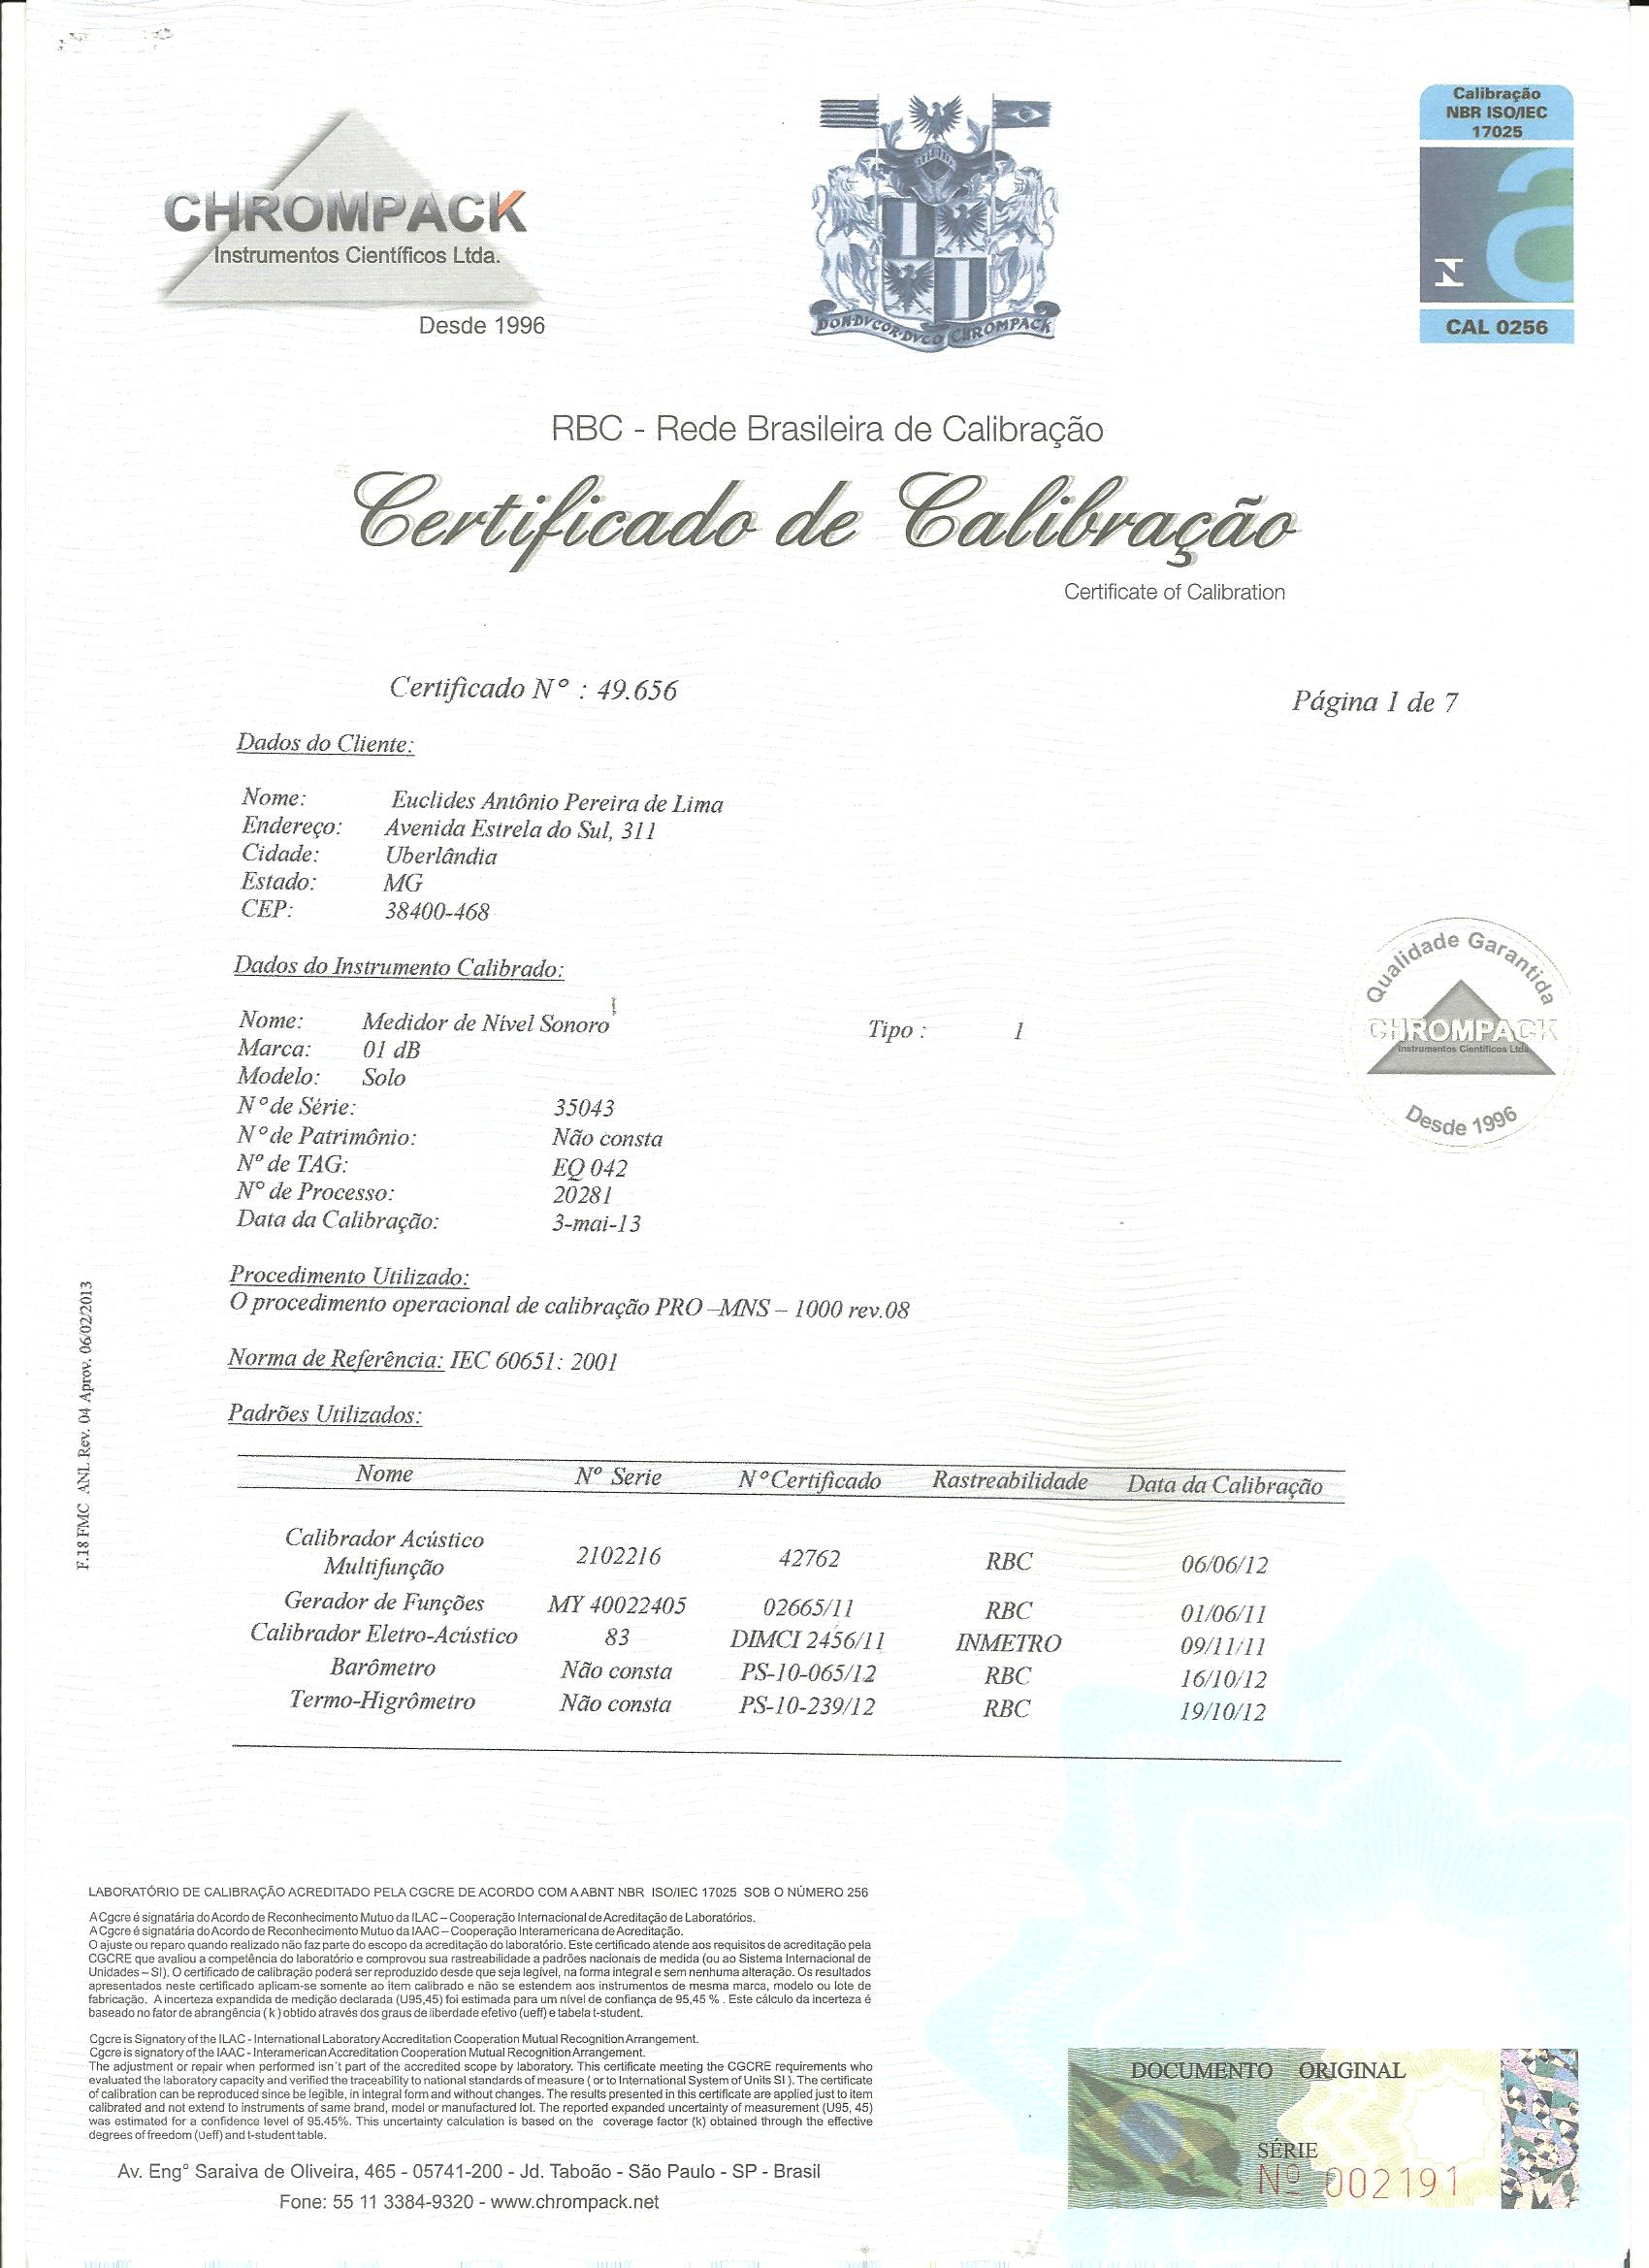
\includegraphics[width=0.9\linewidth]{temp/imagens/anexo3/01.jpg}

\

\

\

\newpage
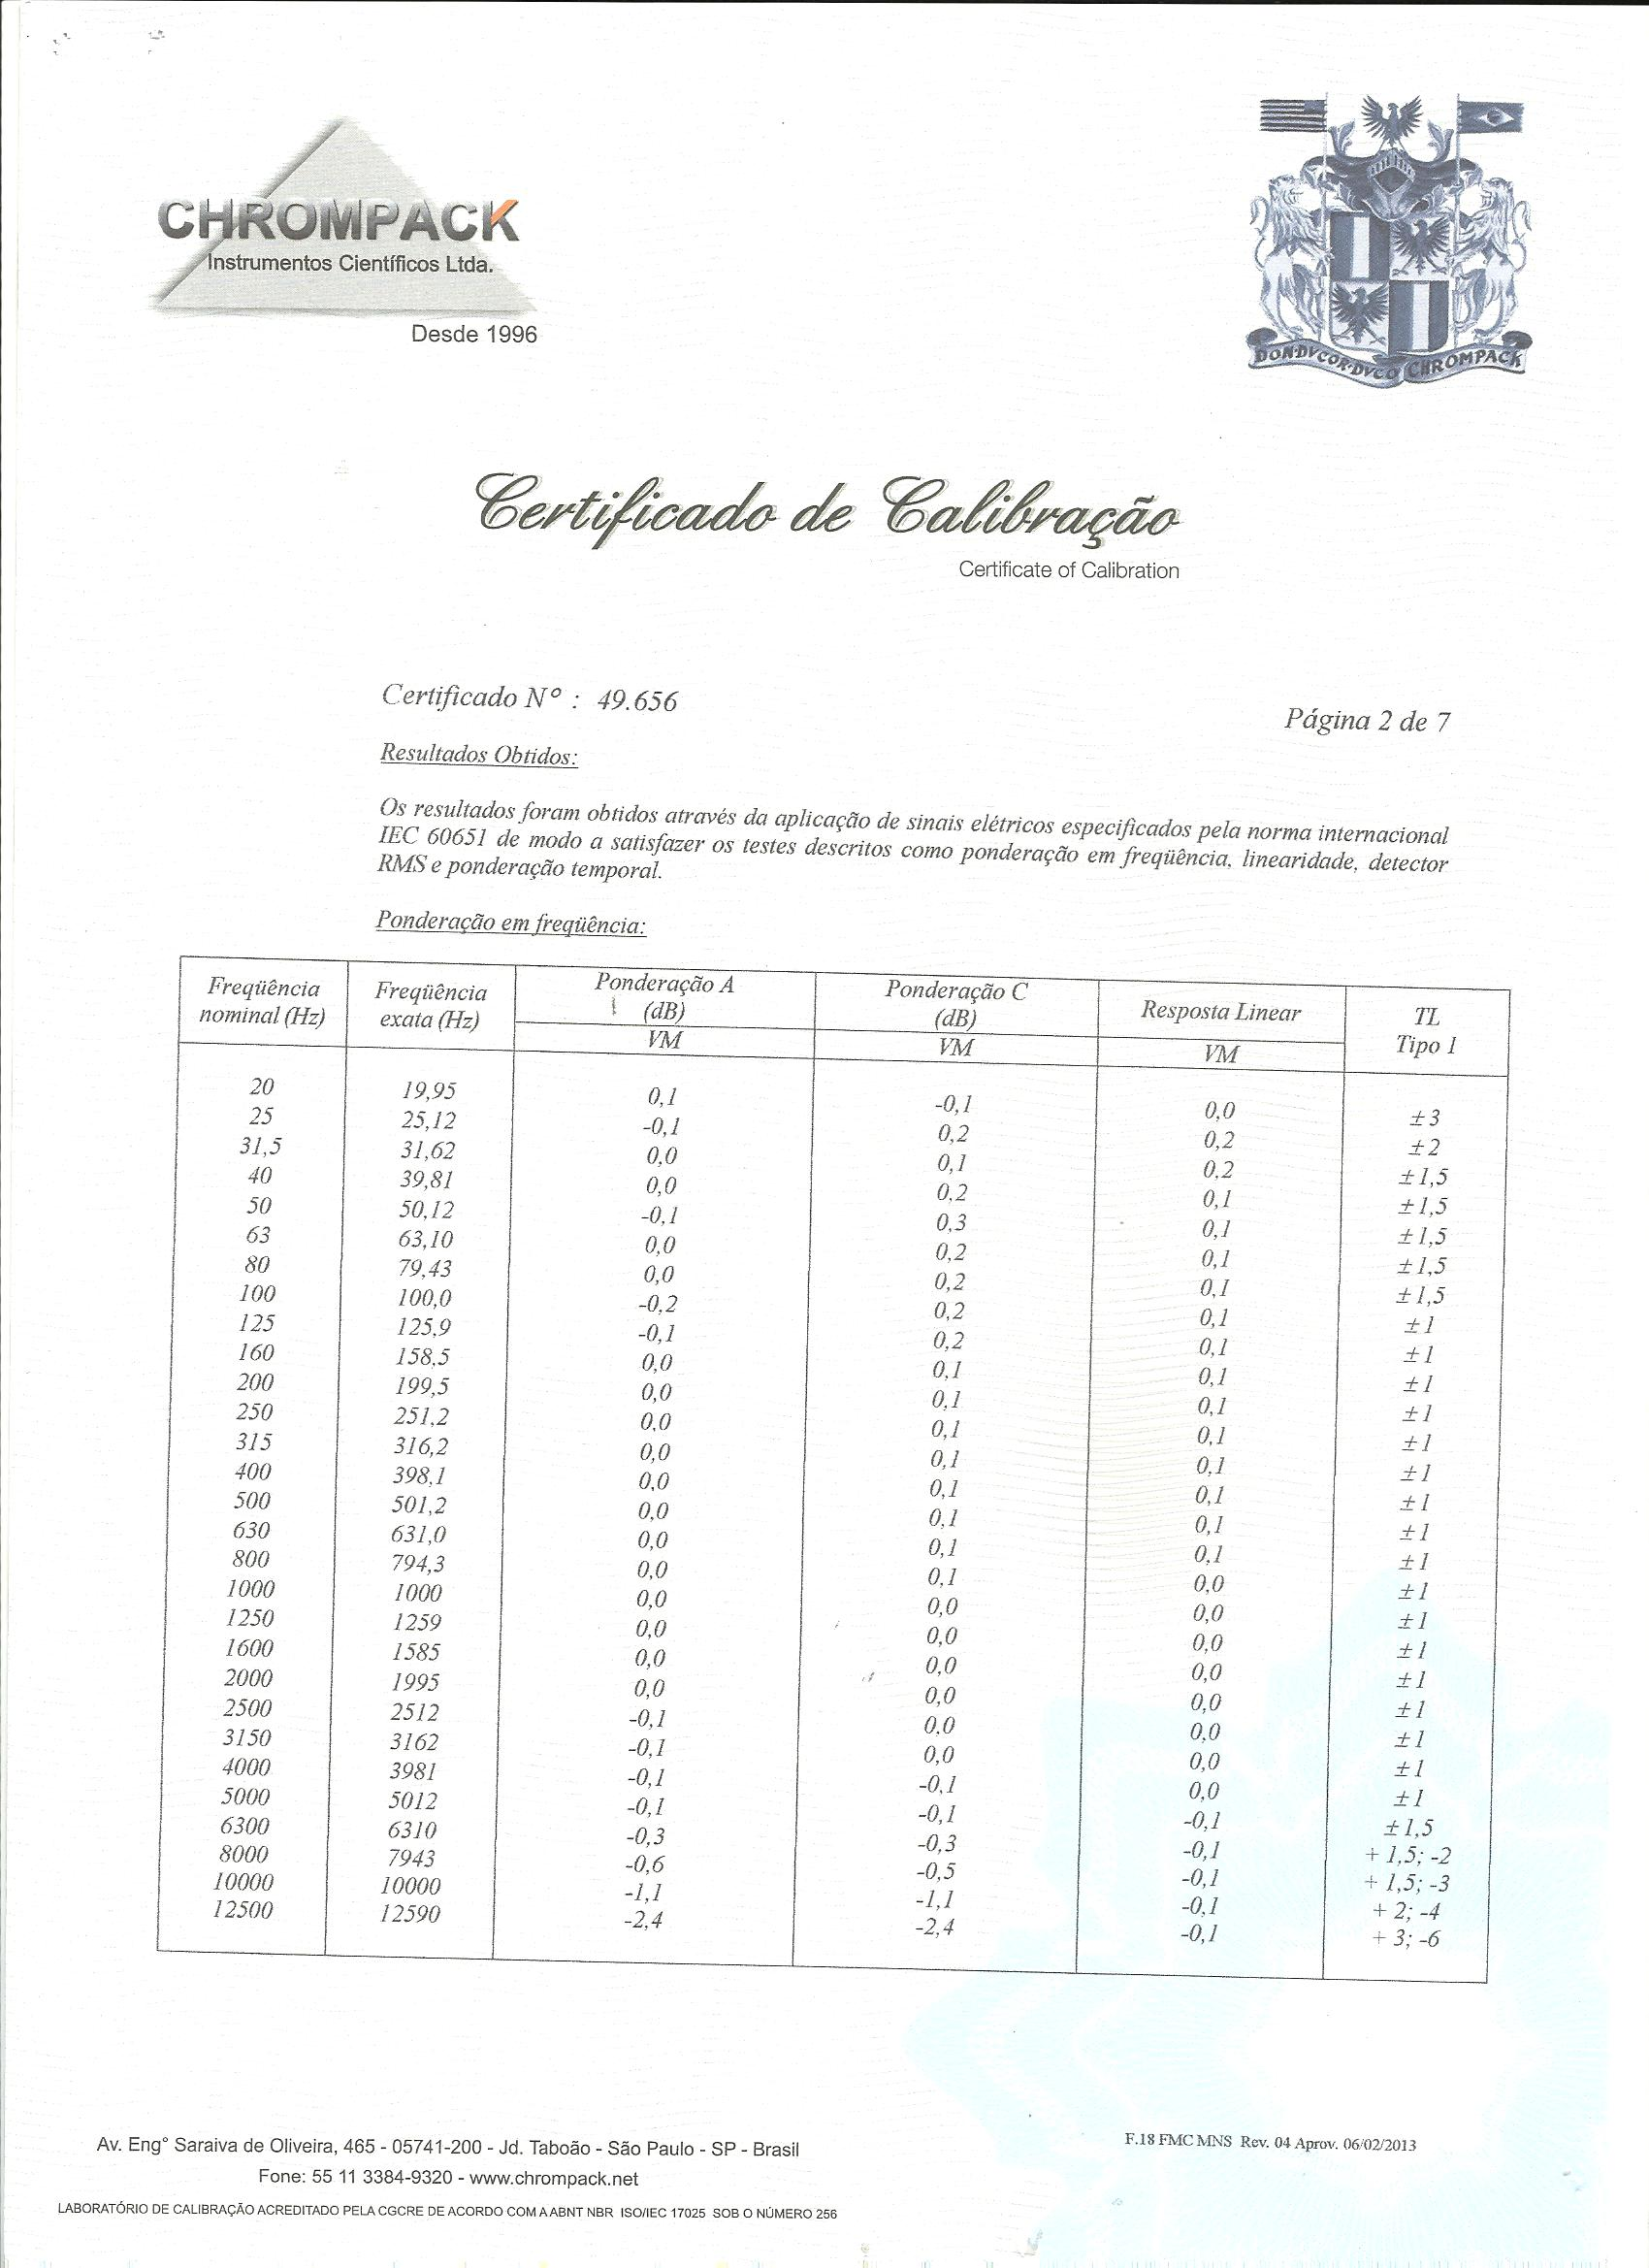
\includegraphics[width=0.9\linewidth]{temp/imagens/anexo3/02.jpg}

\

\

\

\newpage
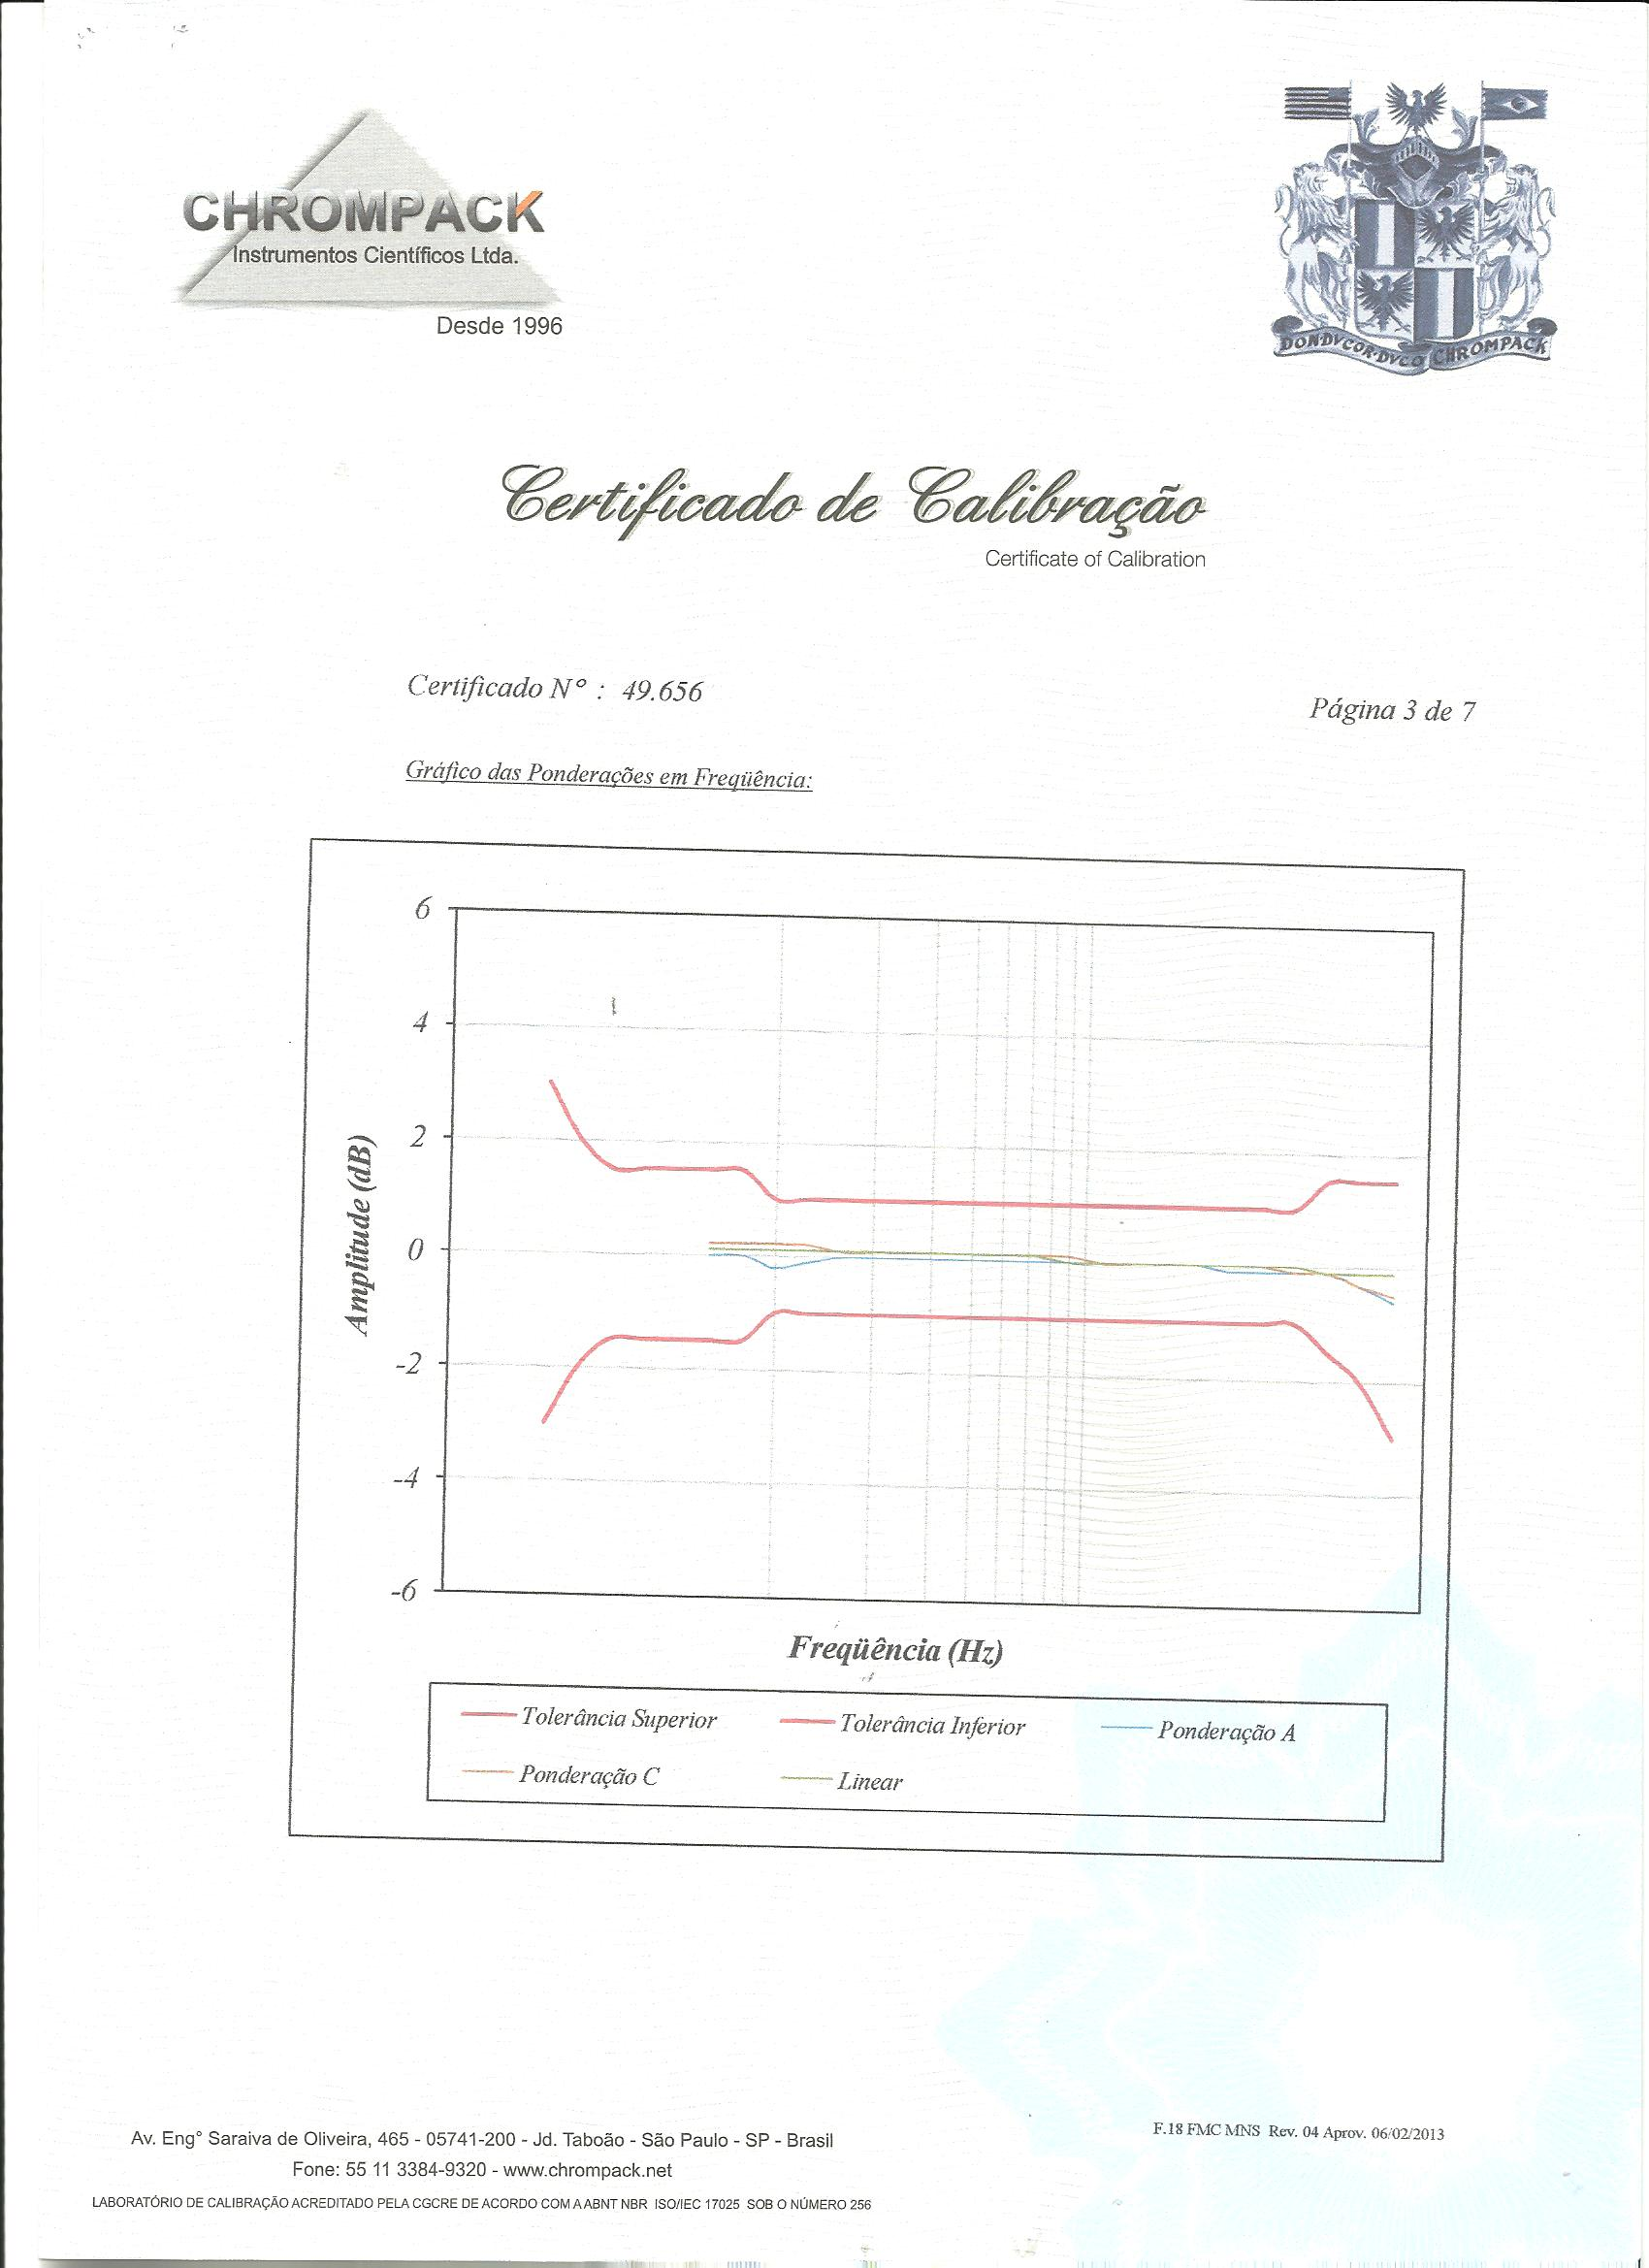
\includegraphics[width=0.9\linewidth]{temp/imagens/anexo3/03.jpg}

\

\

\

\newpage
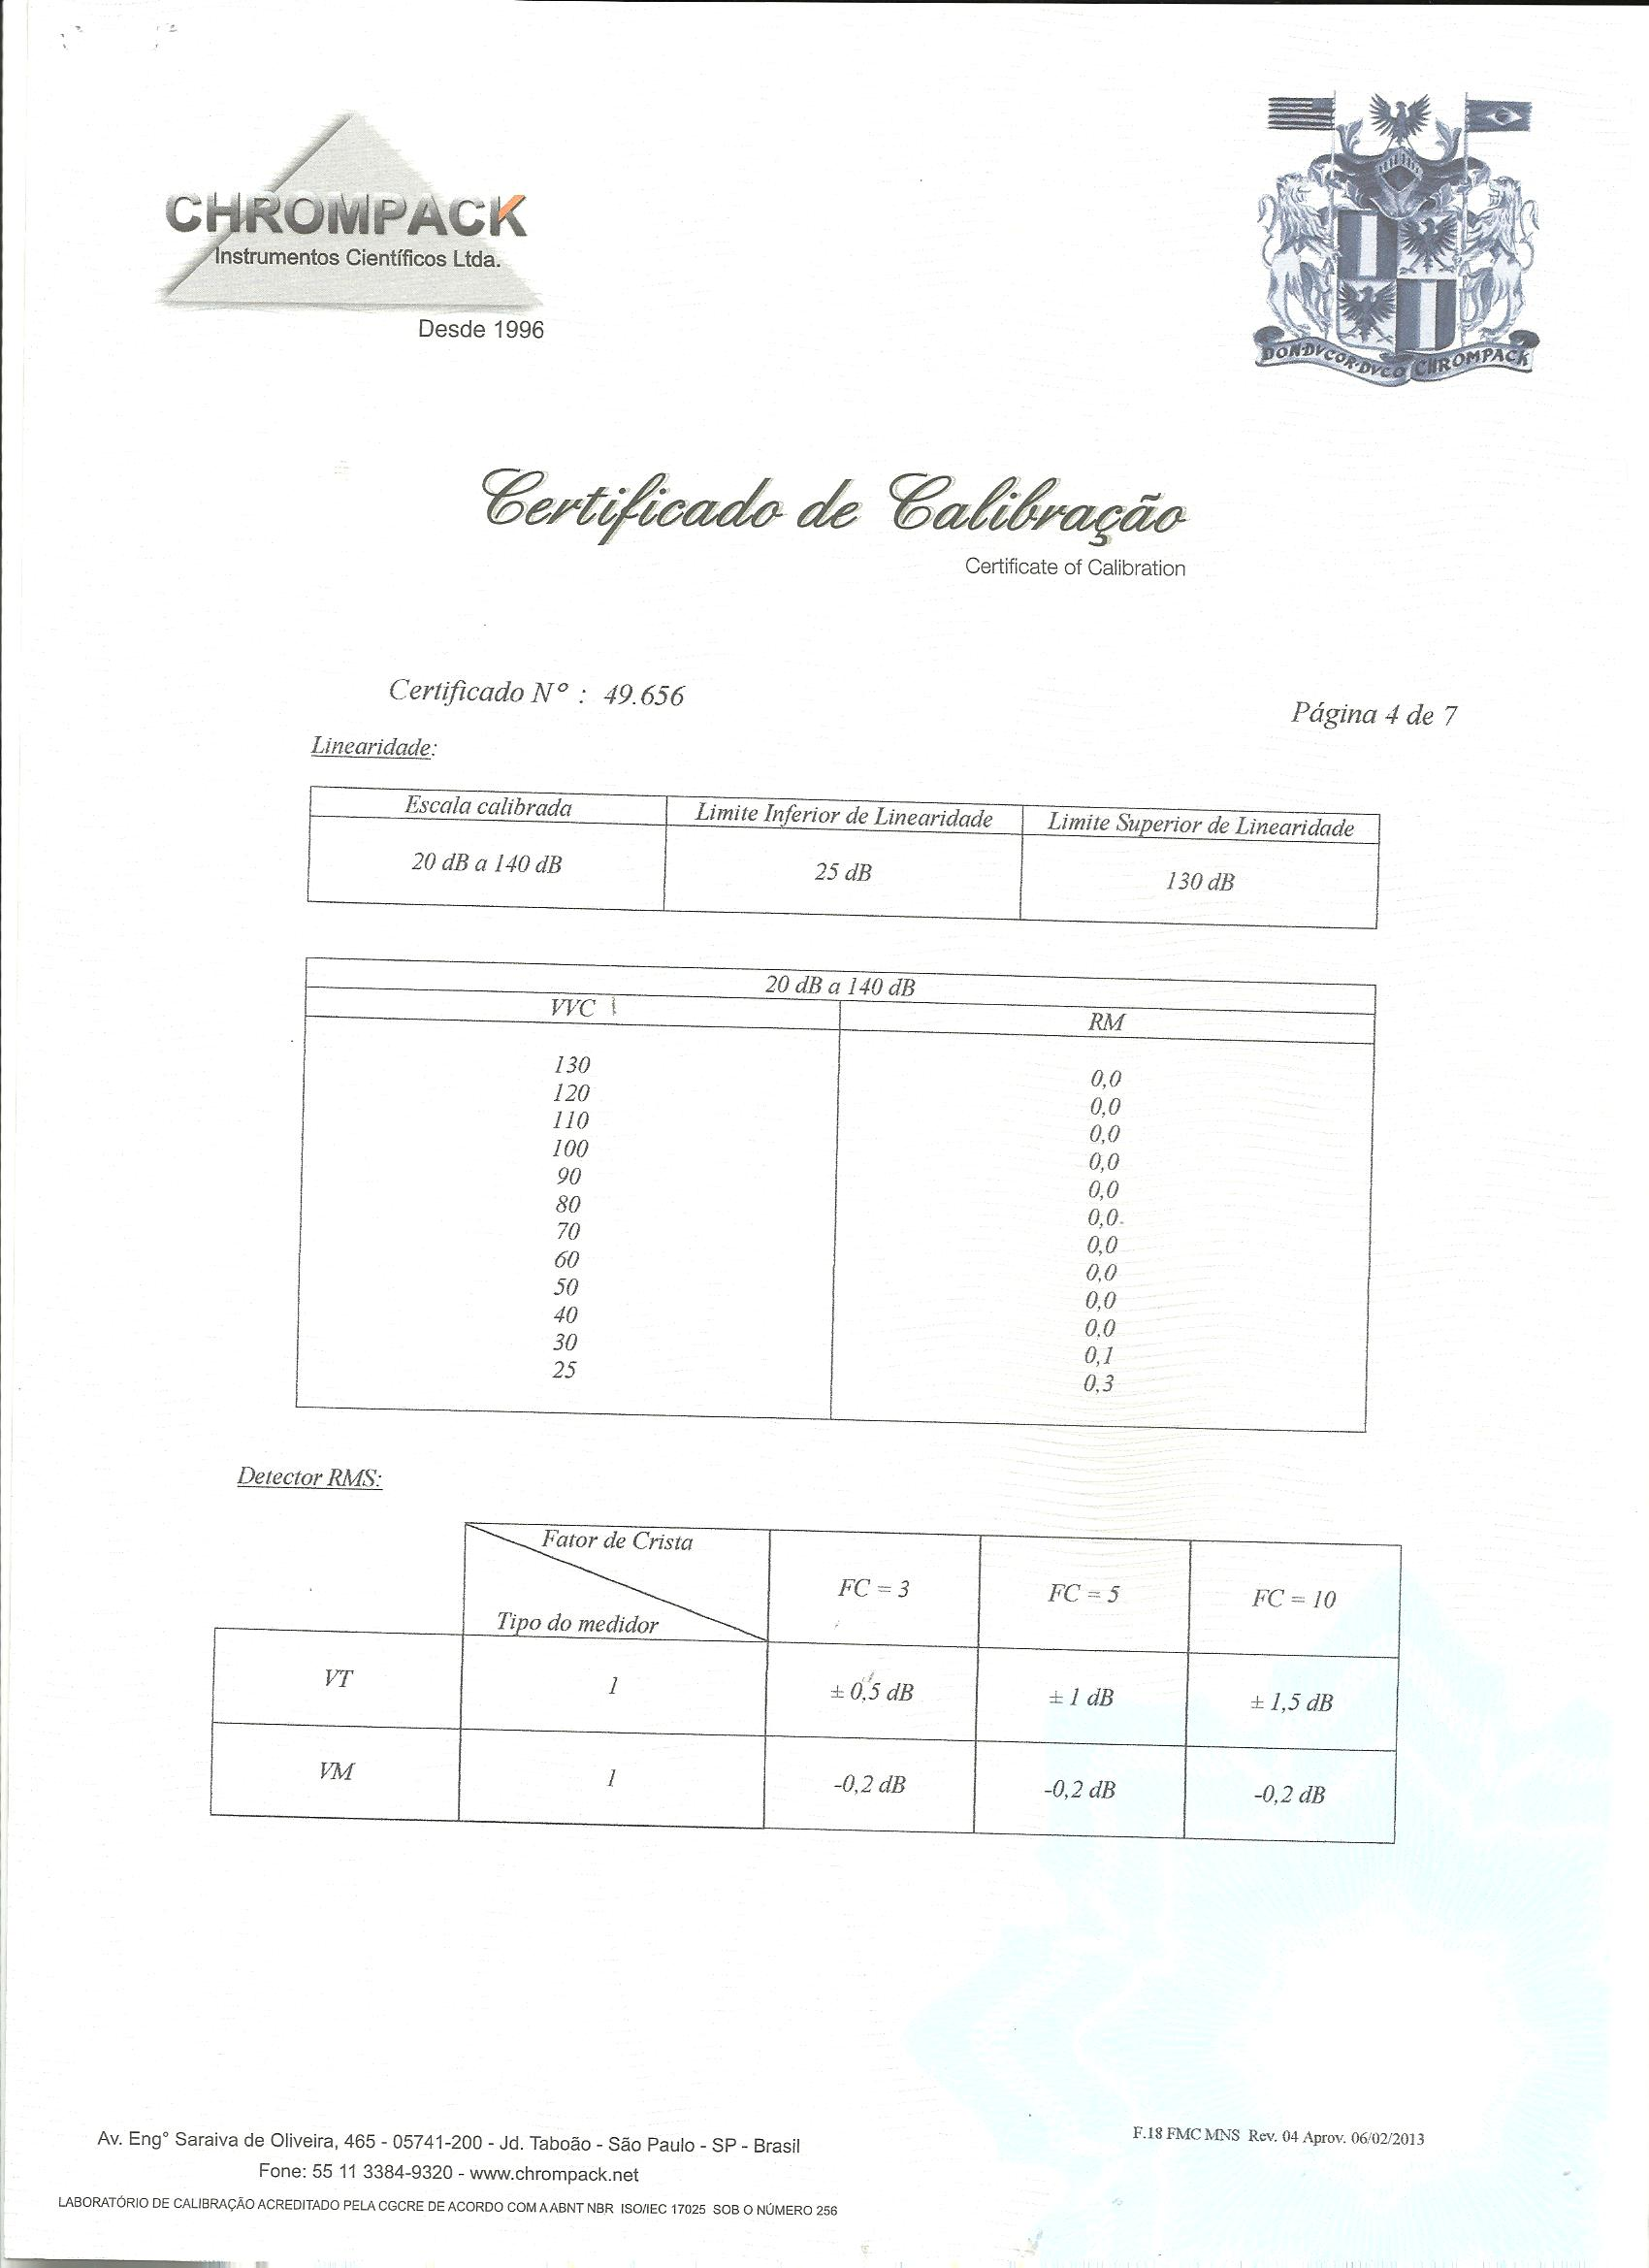
\includegraphics[width=0.9\linewidth]{temp/imagens/anexo3/04.jpg}

\

\

\

\newpage
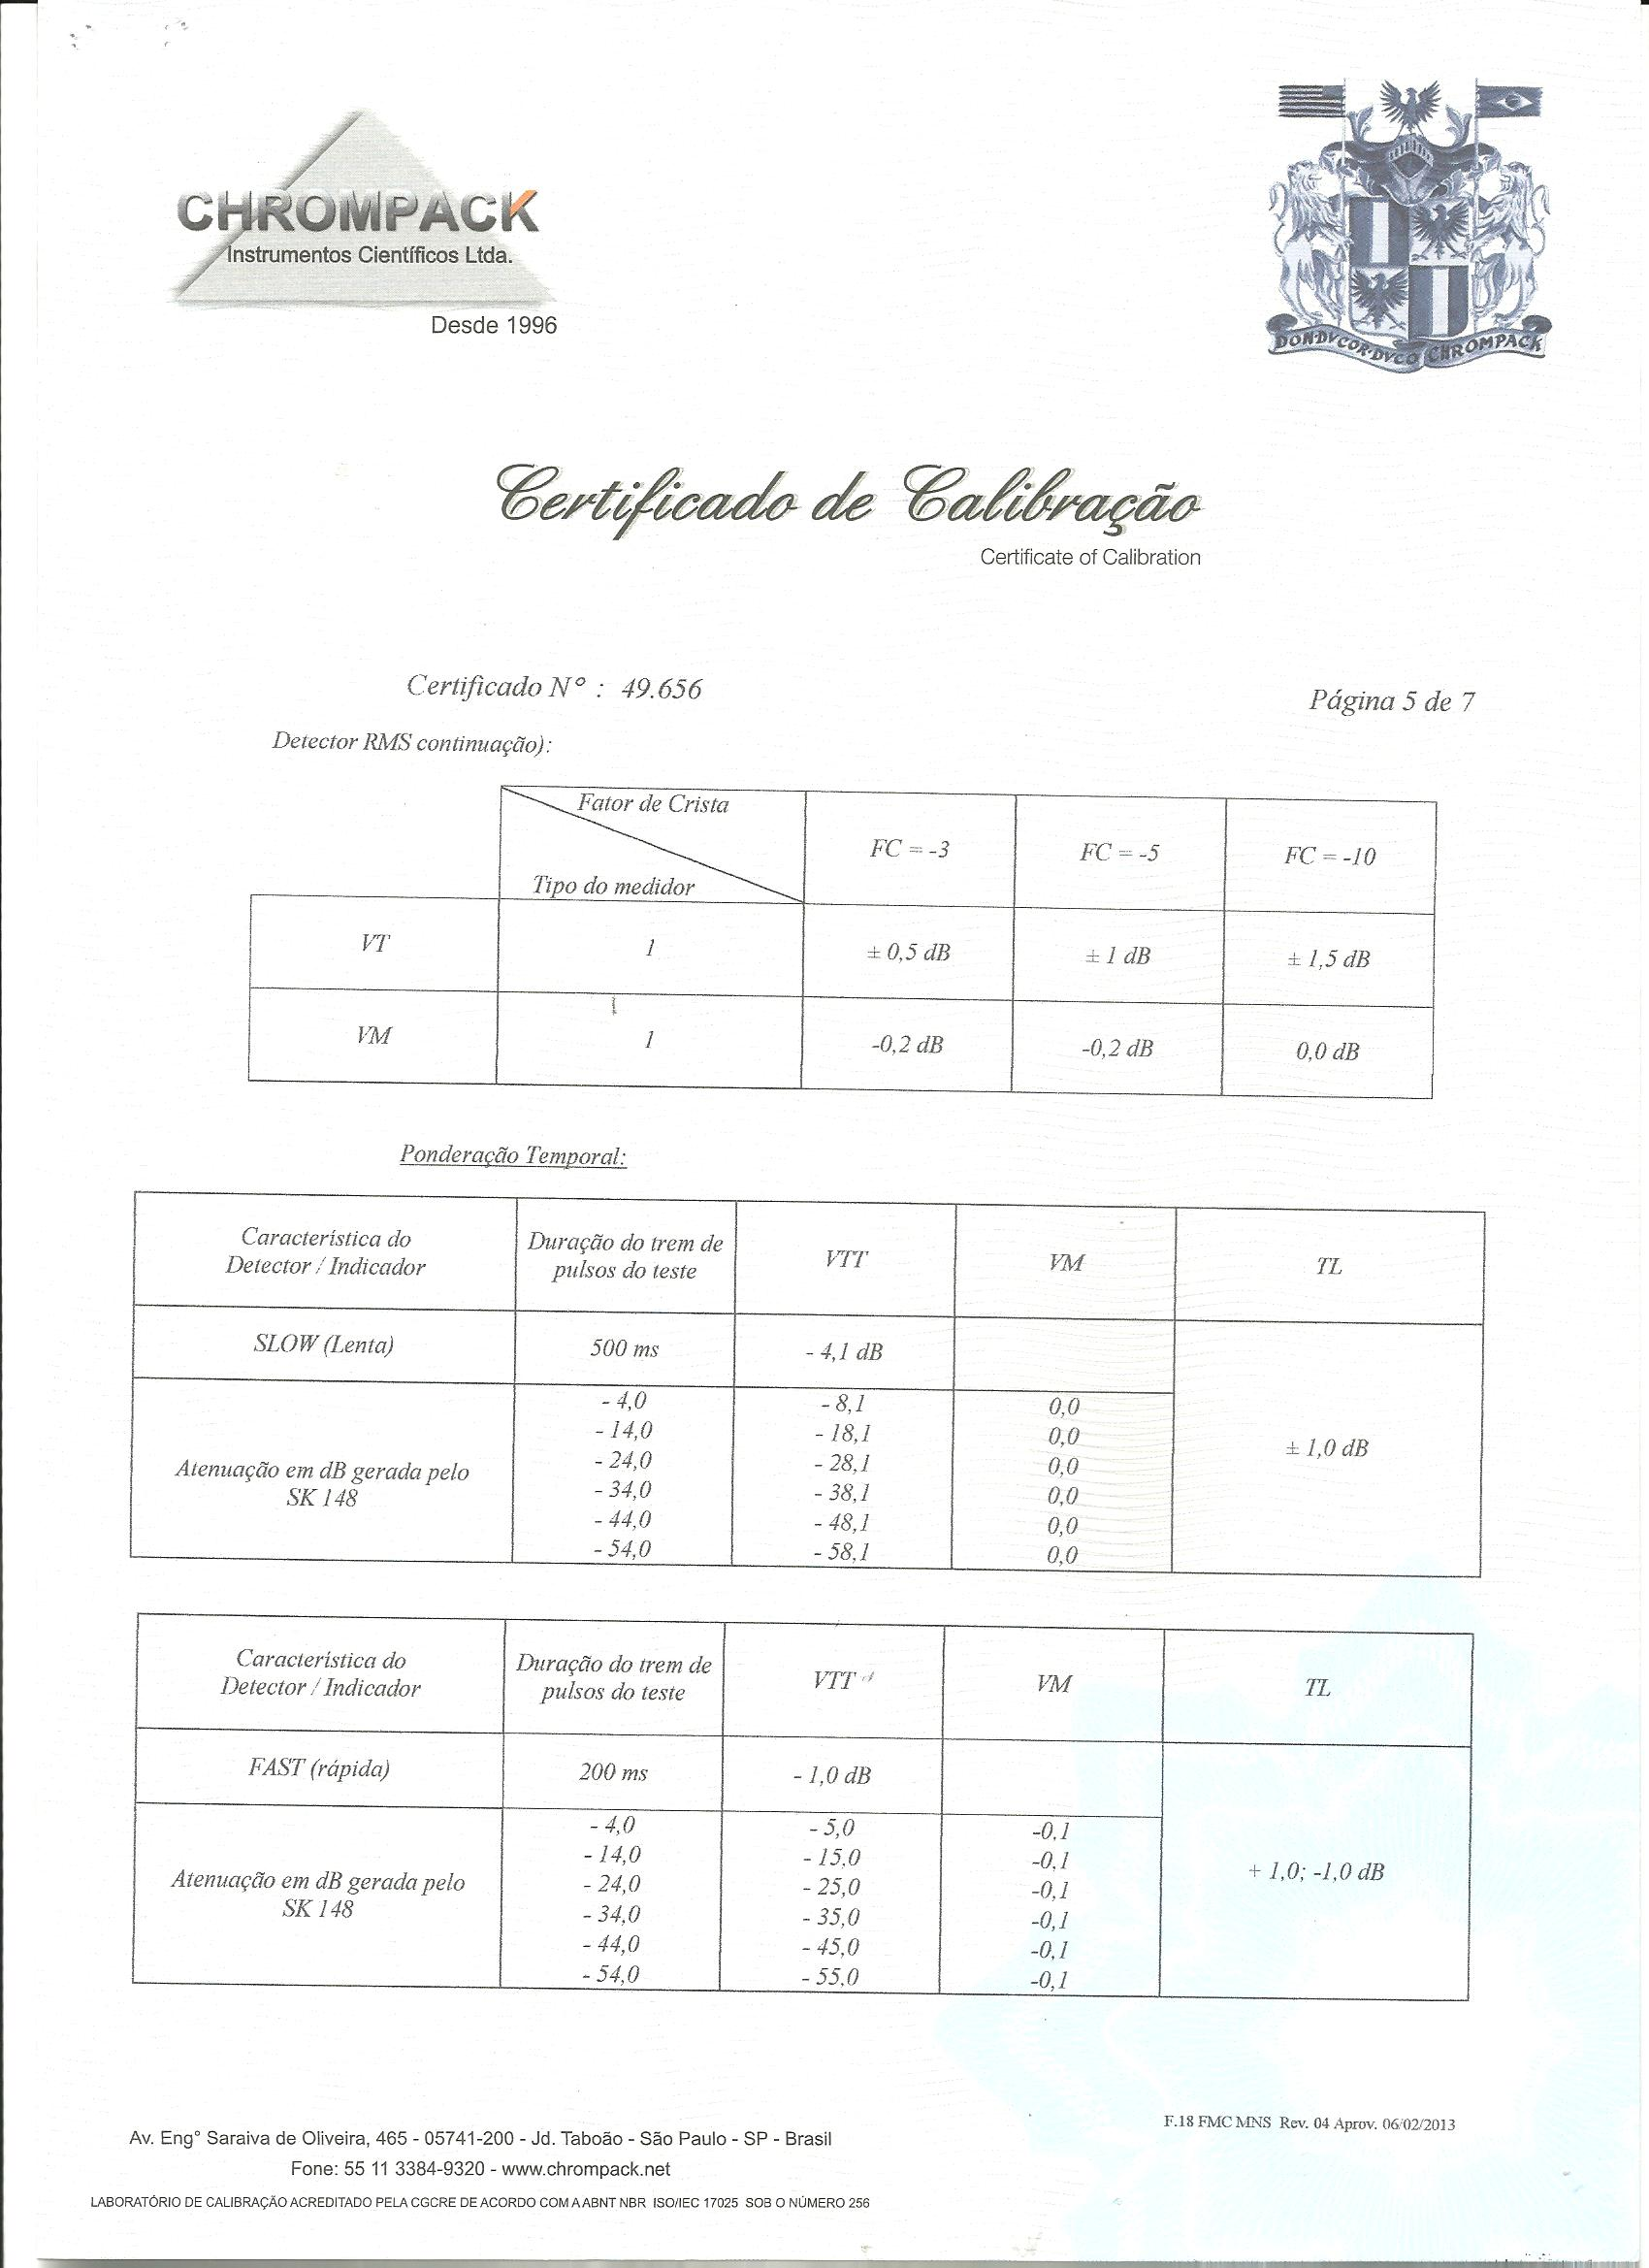
\includegraphics[width=0.9\linewidth]{temp/imagens/anexo3/05.jpg}

\

\

\

\newpage
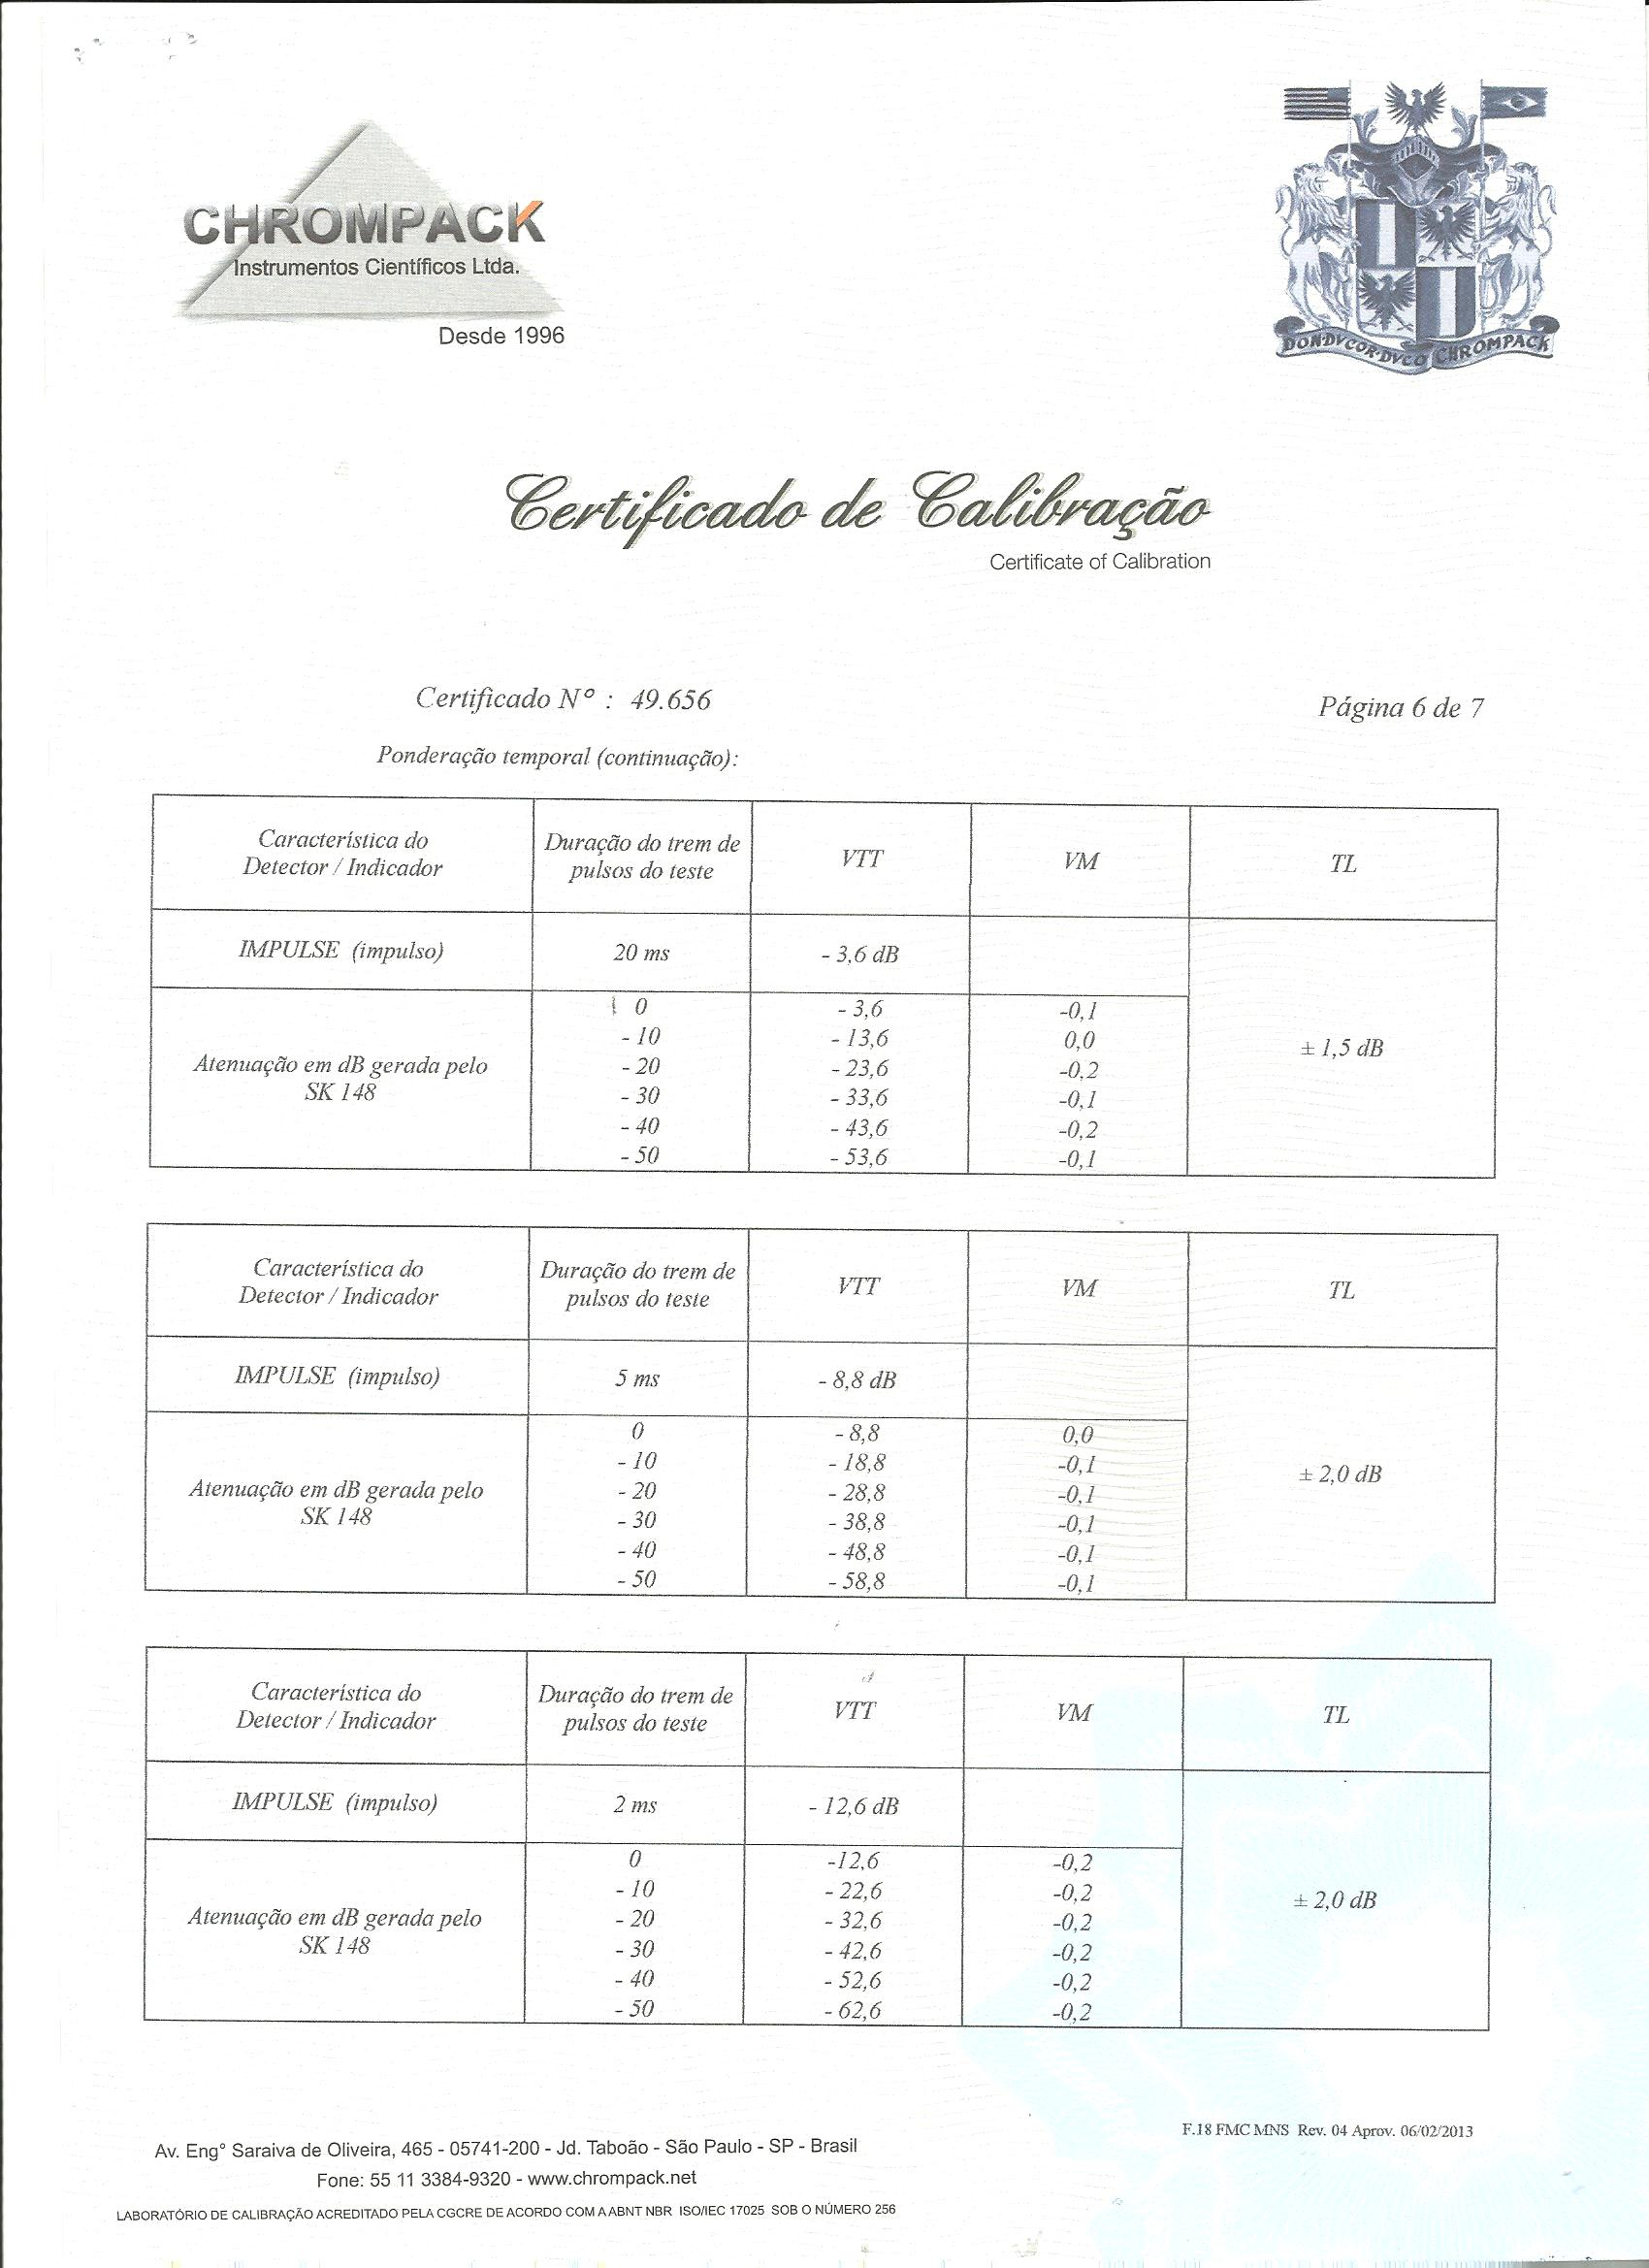
\includegraphics[width=0.9\linewidth]{temp/imagens/anexo3/06.jpg}

\

\

\

\newpage
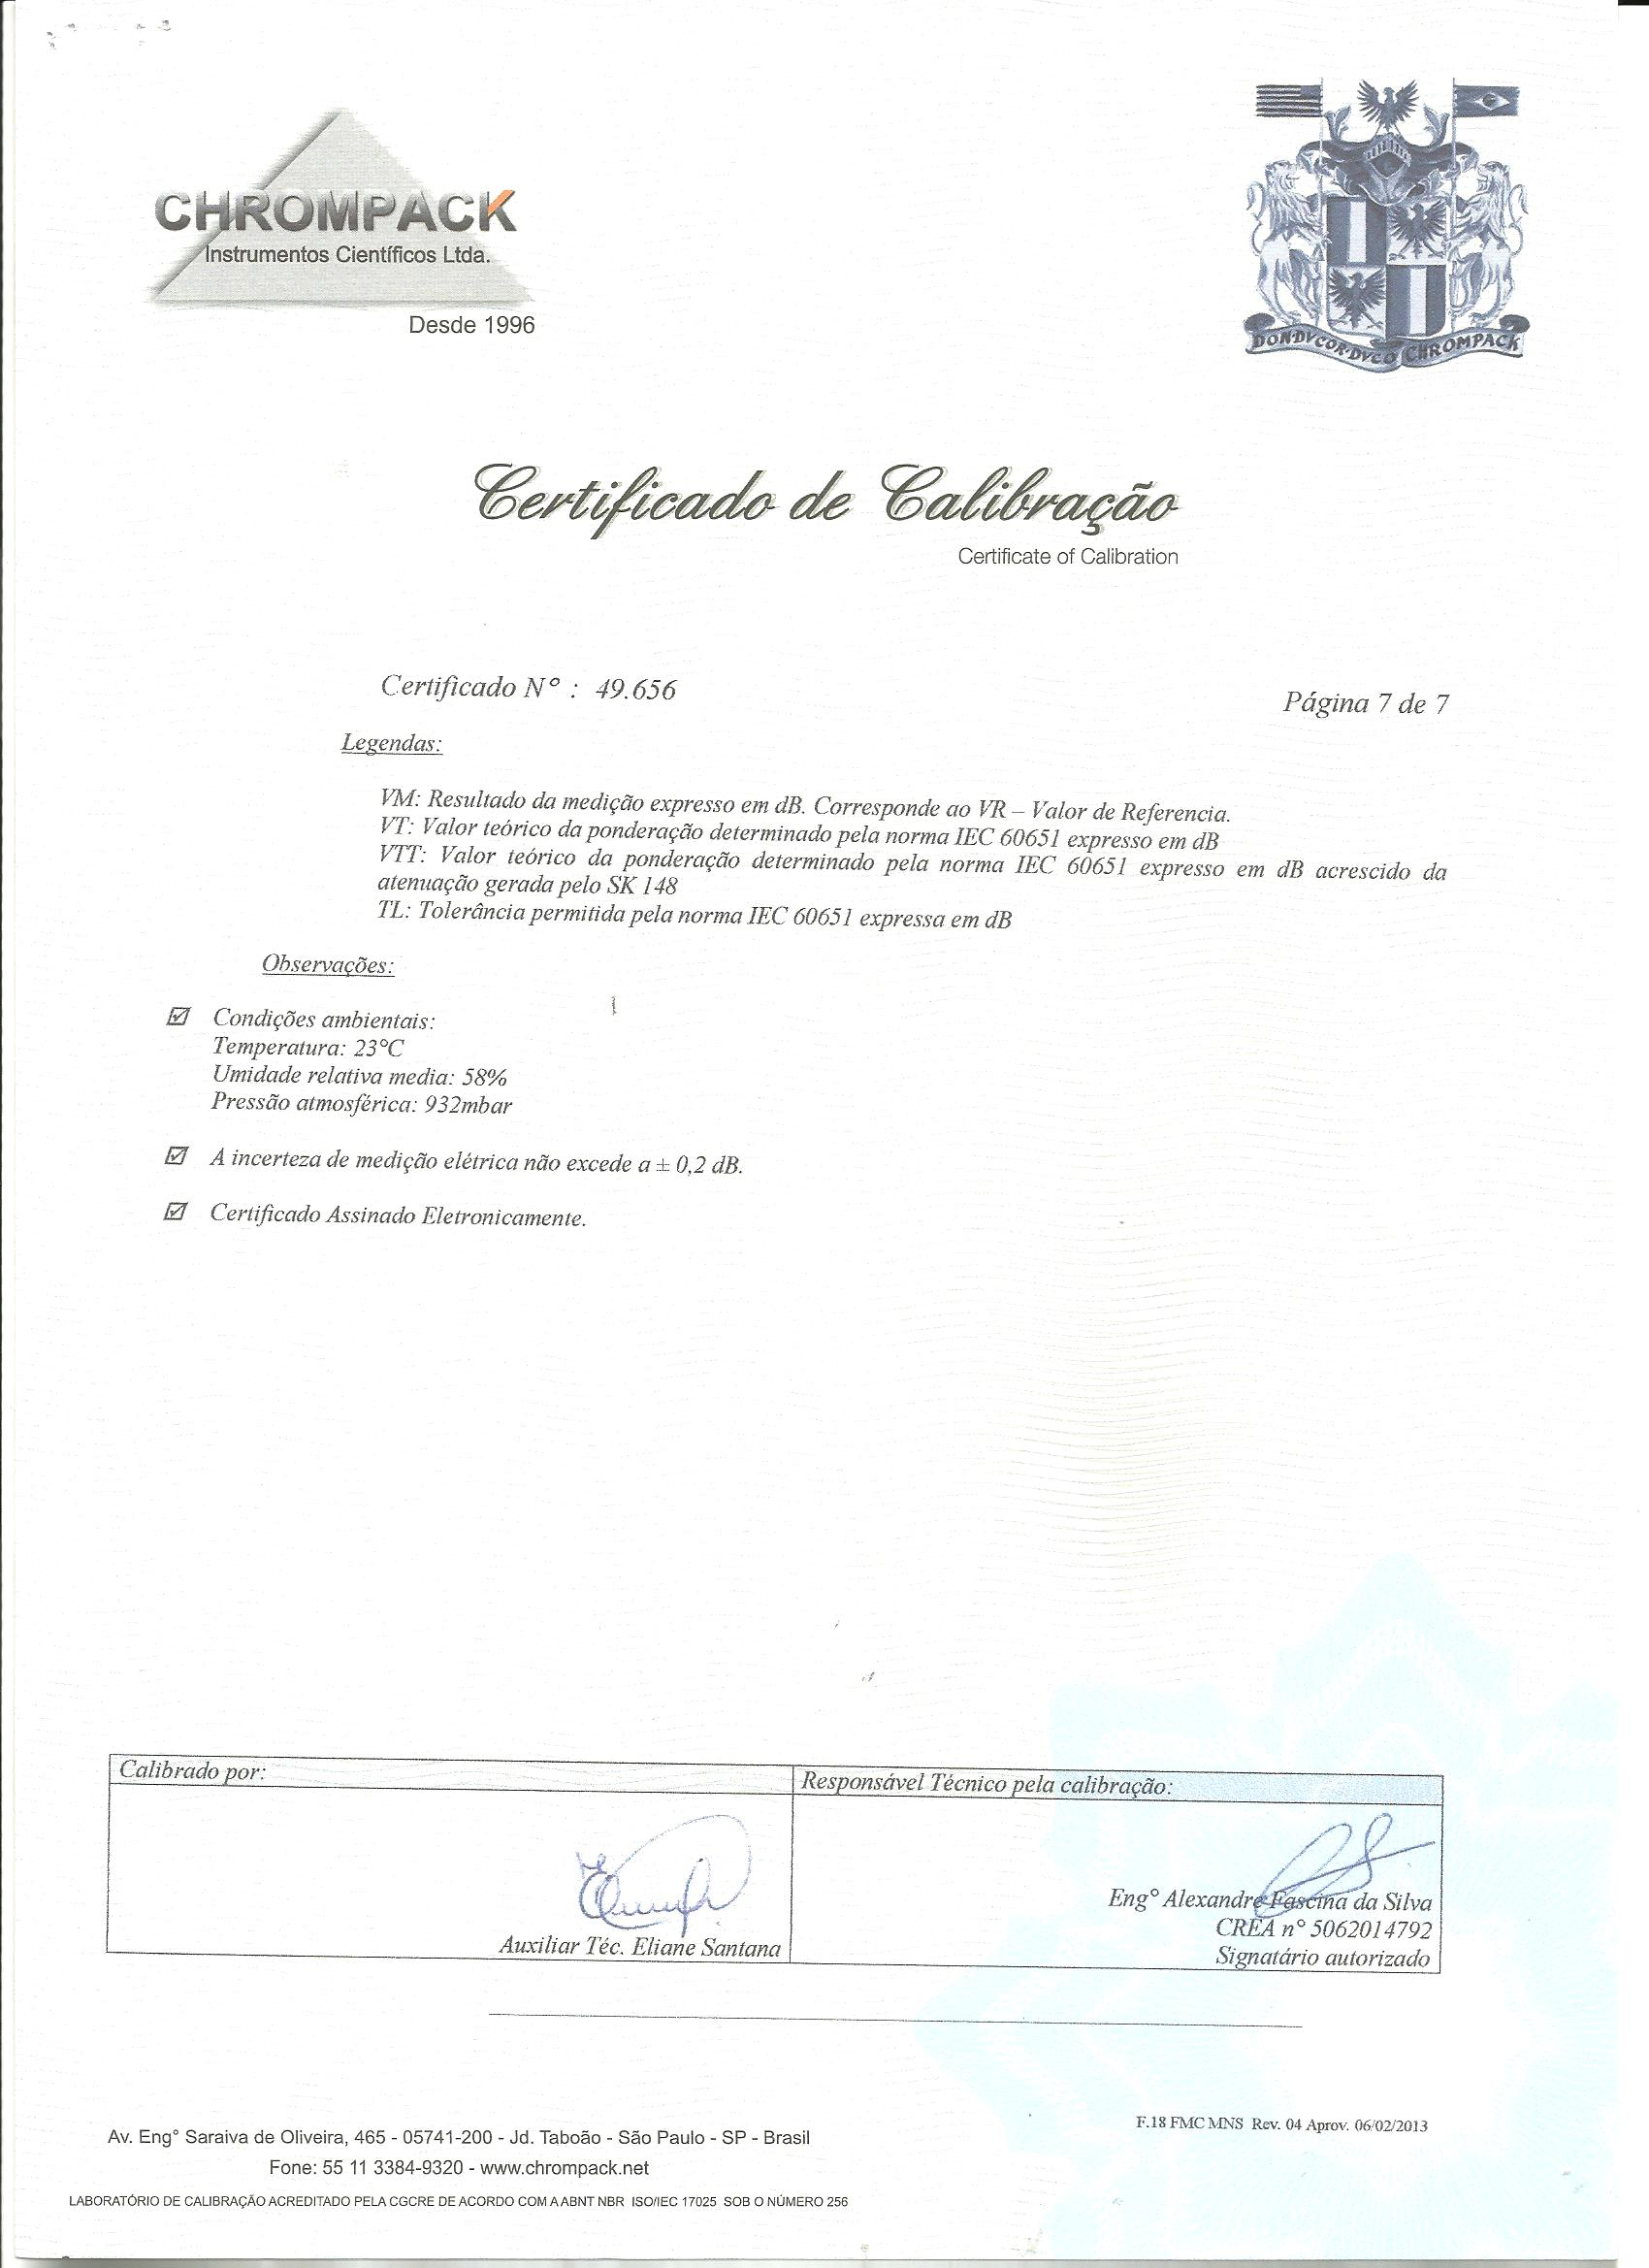
\includegraphics[width=0.9\linewidth]{temp/imagens/anexo3/07.jpg}
\anexo{CERTIFICADO DE PARTICIPAÇÃO NO CURSO DA ASSOCIAÇÃO BRASILEIRA DE NORMAS TÉCNICAS SOBRE A NORMA BRASILEIRA DE REGULAMENTAÇÃO - NBR 10151 / 2000}

\

\

\

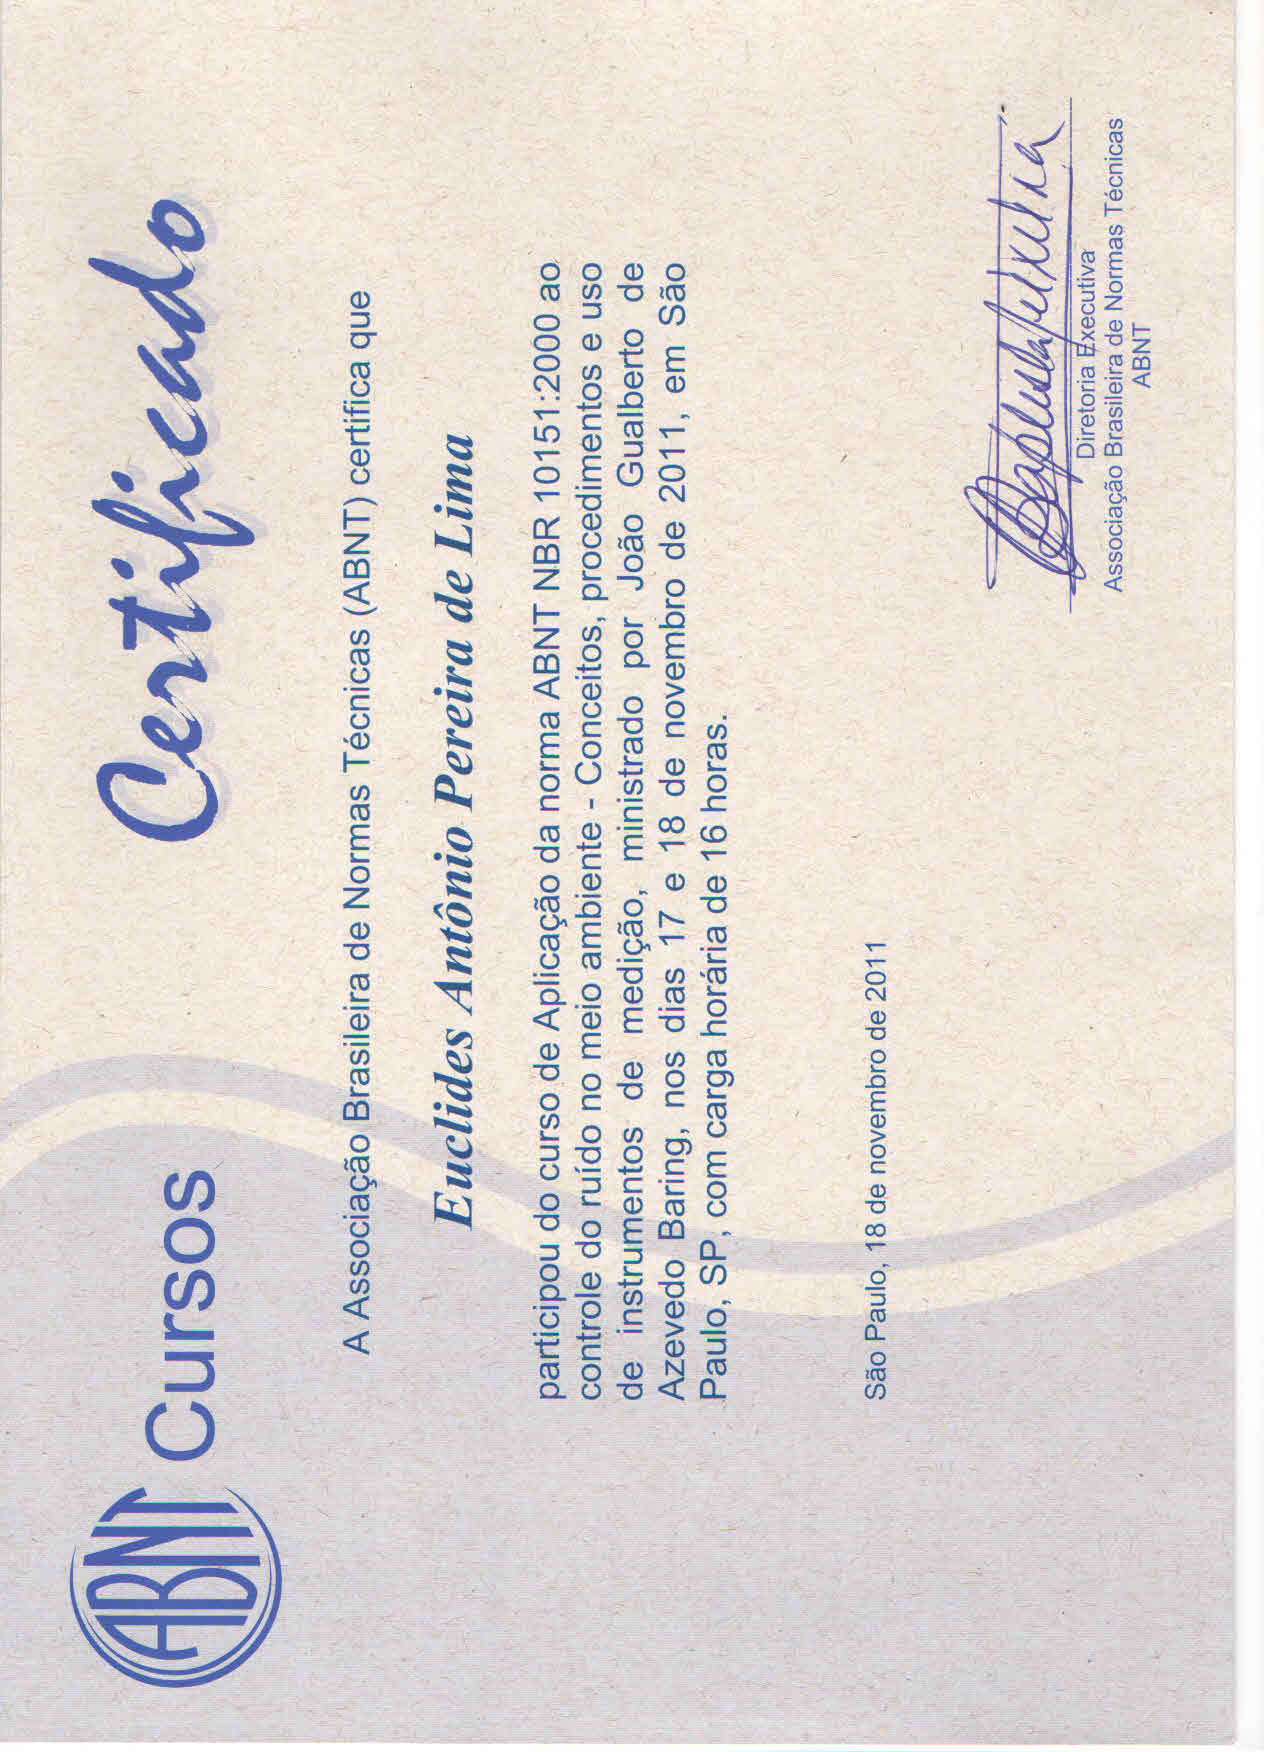
\includegraphics[width=0.9\linewidth]{temp/imagens/anexo4/01.jpg}
\anexo{ANOTAÇÃO DE RESPONSABILIDADE TÉCNICA}
\addtocounter{page}{1}
